%% Type de document et encodage de la police
\documentclass[a4paper]{article}
\usepackage[utf8x]{inputenc}
\usepackage[T1]{fontenc}
% \usepackage[french]{babel}

%% Initialise la taille des pages et des marges
\usepackage[a4paper, top=3cm, bottom=3cm, left=2cm, right=2cm, marginparwidth=2cm]{geometry}

%% Commandes perso
\renewcommand{\arraystretch}{1.2} %% row 20% longer

%% Pour les exemples
\usepackage{mdframed}
\newmdenv[topline=false, bottomline=false, rightline=false, skipabove=\topsep, skipbelow=\topsep]{example}

%% Pour les diagrammes
\usepackage{tikz}
\tikzstyle{incolore} = [rectangle, rounded corners, draw=black, minimum height=1cm, minimum width=3cm, text width=3cm, text centered]

%% Packs utiles
\usepackage{amsmath}
\usepackage{graphicx}
\usepackage{multirow}
\usepackage{float}


\title{Notes Labo Réseaux Q2}
\author{Grégoire Roumache}
\date{Février 2020}

\begin{document}

\maketitle















\section{Labo 1 --- machines virtuelles}





\begin{itemize}





\item Topologie:
\begin{center}
    \begin{tikzpicture}
        \node (servg) [] at (0,0) {
\includegraphics[height=1.5cm]{images/ibm_tower.jpg}};
        \node (routg) [] at (4,0) {
\includegraphics[width=1.5cm]{images/router.jpg}};
        \node (routd) [] at (8,0) {
\includegraphics[width=1.5cm]{images/router.jpg}};
        \node (servd) [] at (12,0) {
\includegraphics[height=1.5cm]{images/ibm_tower.jpg}};

        \draw [thick, blue]  (servg) -- node[anchor=south]{\begin{tabular}{c} IntNetG \\ 192.168.1.0/24 \end{tabular}} (routg);
        \draw [thick, red]   (routg) -- node[anchor=south]{\begin{tabular}{c} IntNetC \\ 10.0.0.0/30 \end{tabular}} (routd);
        \draw [thick, green] (routd) -- node[anchor=south]{\begin{tabular}{c} IntNetD \\ 192.168.2.0/24 \end{tabular}} (servd);

        \node [] at (0,-1.25) {serveur g.};
        \node [] at (4,-1.25) {routeur g.};
        \node [] at (8,-1.25) {routeur d.};
        \node [] at (12,-1.25) {serveur d.};
    \end{tikzpicture}
\end{center}





\item Remarque: les routeurs doivent avoir 2 interfaces, 1 pour chaque réseau.





\item Liste des commandes de base utilisées:
\begin{itemize}
    \item \texttt{ip a}: affiche le nom des interfaces et permet de vérifier si les ip ont bien étées attribuées.
    \item \texttt{nano /etc/network/interfaces}: nano perme d'éditer le fichier.
    \item \texttt{systemctl restart networking}: redémarre le service réseau.
    \item \texttt{reboot}: en cas de problème avec la commandes ci-dessus.
    \item \texttt{traceroute <ip>}: affiche le chemin entre la machine et l'ip donnée.
    \item \texttt{route}: affiche la table de routage.
\end{itemize}





\item Implémentation du routage:
\begin{itemize}
    \item Configuration temporaire (1):
    \begin{itemize}
        \item \texttt{sysctl -w net.ipv4.ip\_forward=1}: configuration temporaire qui permet le routage.
    \end{itemize}
    \item Configuration temporaire (2):
    \begin{itemize}
        \item \texttt{ip route add <ip>/<masque> via <ip> dev <interface>}
    \end{itemize}
    \item Configuration permanente:
    \begin{enumerate}
        \item éditer le fichier: \texttt{/etc/sysctl.conf},
        \item décommenter la ligne: \texttt{net.ipv4.ip\_forward=1},
        \item redémarrer le service: \texttt{sysctl -p /etc/sysctl.conf}.
    \end{enumerate}
\end{itemize}





\item Exemple de configuration réseau à mettre en place (routeur g.):
\begin{verbatim}
auto enp0s3
iface enp0s3 inet static
    address 192.168.1.254
    netmask 255.255.255.0

auto enp0s8
iface enp0s8 inet static
    address 10.0.0.1
    netmask 255.255.255.252
    gateway 10.0.0.2
\end{verbatim}





\end{itemize}















\newpage \section{Labo 2 --- routage sur routeur RouterOS}





\begin{itemize}





% \item NOTES (avant la manip):
% \begin{itemize}
%     \item Étapes de la manipulation:
%     \begin{enumerate}
%         \item Reset des RouterOS:
%         \begin{enumerate}
%             \item Pressez le bouton \textit{reset} avant de brancher l’alimentation.
%             \item Le garder enfoncé jusqu'à l'extinction de la LED \textit{ACT}.
%             \item Le routeur a l'adresse \texttt{192.168.88.1}, c'est aussi un serveur DHCP.
%         \end{enumerate}
%         \item Câblage de l’infrastructure:
%         \begin{enumerate}
%             \item Connectez donc le port 2 de votre RouterOS à la carte ethernet de votre PC.
%             \item Configurez votre PC en DHCP et vérifiez que son adresse est sur le réseau 192.168.88.0/24.
%             \item Tester la connection au routeur avec: \texttt{ping 192.168.88.1}.
%             \item Ouvrir un browser et se connecter vers: \texttt{192.168.88.1/webfig/\#Quick\_Set}.
%             \item Le login est \textit{admin} et le mot de passe est vide.
%         \end{enumerate}
%         \item Configuration des RouterOS et des PC’s clients:
%         \begin{enumerate}
%             \item Se connecter au routeur avec Putty en SSH à l'adresse: \texttt{192.168.88.1}.
%             \item Tester les commandes suivantes:
%             \begin{itemize}
%                 \item \texttt{/ip address print}
%                 \item \texttt{/interface print}
%                 \item \texttt{/ip route print}
%             \end{itemize}
%             \item Supprimer la configuration d’usine: \texttt{/system reset-configuration no-defaults=yes}
%         \end{enumerate}
%         \item Test de l’interconnexion des réseaux:
%         \item Test de l’accès à internet:
%     \end{enumerate}
% \end{itemize}





% (Après la manip)
\item Étapes de la manipulation:
\begin{enumerate}


    \item Reset des RouterOS.
    \begin{example}
        \begin{enumerate}
            \item Pressez le bouton \textit{RES} (= reset) avant de brancher l’alimentation.
            \item Le garder enfoncé jusqu'à l'extinction de la LED \textit{ACT}.
            \item Le routeur a l'adresse \texttt{192.168.88.1}, c'est aussi un serveur DHCP.
        \end{enumerate}
    \end{example}


    \item Câblage de l’infrastructure.
    \begin{example}
        \begin{center}
            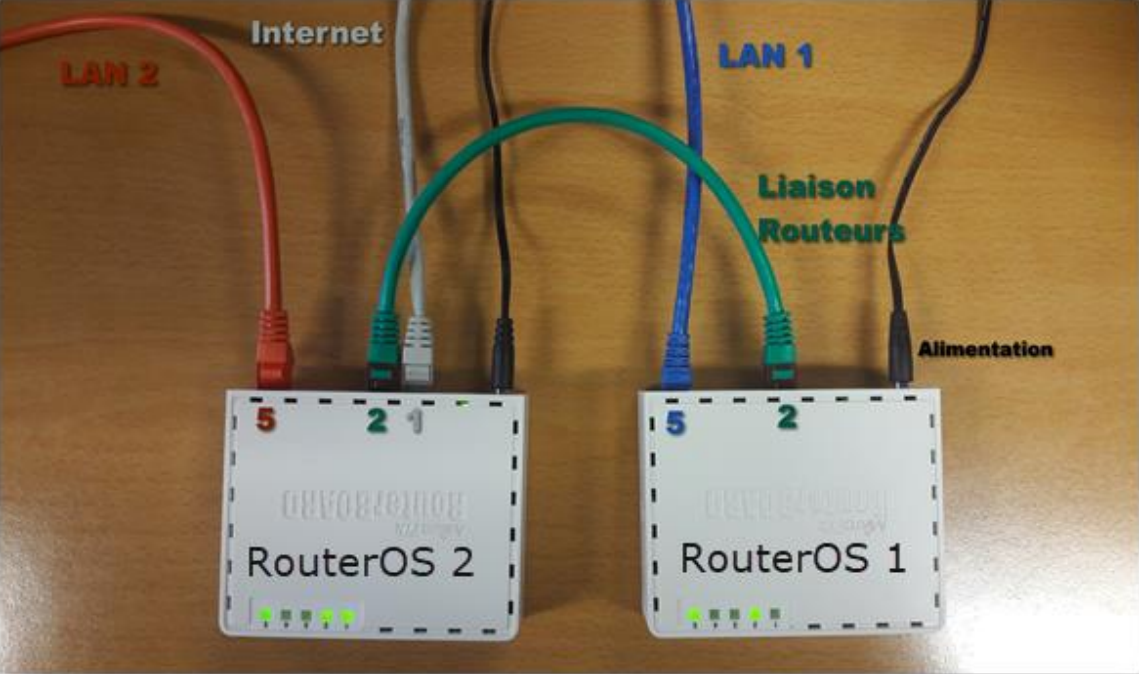
\includegraphics[width=0.95\textwidth]{images/cablage-RouteurOS.PNG}
        \end{center}
        \begin{enumerate}
            \item Brancher le câble vert de chaque PC dans un routeur (port 5).
            \item Brancher les 2 routeurs ensembles (port 2).
            \item Débrancher le câble ethernet de l'ordinateur pour connecter le routeur 2 à internet (port 1, \textit{PoE} = power over internet).
        \end{enumerate}
    \end{example}


    \item Configuration des RouterOS (1ère partie).
    \begin{example}
        Pour chaque routeur:
        \begin{enumerate}
            \item Démarrer WinBox, clicker sur la MAC address du routeur puis clicker sur \textit{Connect}.
            \item Dans le menu de gauche, clicker sur \textit{IP}, puis sur \textit{Addresses}.
            \item Dans la fenêtre qui vient de s'ouvrir, clicker sur le \textcolor{blue}{\textbf{+}} bleu.

            \item Ensuite, remplir le formulaire:
            \begin{itemize}
                \item Routeur 1:
                \begin{itemize}
                    \item dans \textit{Addresses}, mettre: \texttt{192.168.1.1/24},
                    \item dans \textit{Interface}, mettre: \texttt{ether5}.
                \end{itemize}

                \item Routeur 2:
                \begin{itemize}
                    \item dans \textit{Addresses}, mettre: \texttt{192.168.2.1/24},
                    \item dans \textit{Interface}, mettre: \texttt{ether5}.
                \end{itemize}
            \end{itemize}

            \item Clicker sur \textit{OK}.
            \item Dans le menu de gauche, clicker sur \textit{System}, puis sur \textit{Identity}.
            \item Mettre le nom du routeur dans le champ \textit{Identity} (RouterOS1 ou RouterOS2).
            \item Clicker sur \textit{OK}.
        \end{enumerate}
    \end{example}


    \item Configuration des PC clients.
    \begin{example}
        \begin{itemize}
            \item Il faut configurer les paramètres réseau en statique.
            \item Pour le PC connecté à RouterOS1:
            \begin{itemize}
                \item adresse = \texttt{192.168.1.2},
                \item masque = \texttt{255.255.255.0},
                \item gateway = \texttt{192.168.1.1},
                \item dns = \texttt{8.8.8.8}.
            \end{itemize}
            \item Pour le PC connecté à RouterOS2:
            \begin{itemize}
                \item adresse = \texttt{192.168.2.2},
                \item masque = \texttt{255.255.255.0},
                \item gateway = \texttt{192.168.2.1},
                \item dns = \texttt{8.8.8.8}.
            \end{itemize}
        \end{itemize}
    \end{example}


    \item Configuration des RouterOS (2ème partie).
    \begin{example}
        Pour RouterOS1, utiliser les commandes suivantes:
        \begin{enumerate}
            \item \texttt{/ip address}
            \item \texttt{add address=192.168.99.1/24 interface=ether2}
            \item \texttt{/ip route}
            \item \texttt{add gateway=192.168.99.2}
        \end{enumerate}
        Pour RouterOS2, utiliser les commandes suivantes:
        \begin{enumerate}
            \item \texttt{/ip address}
            \item \texttt{add address=192.168.99.2/24 interface=ether2}
            \item \texttt{/ip dhcp-client add interface=ether1 disable=no}
            \item \texttt{/ip route}
            \item \texttt{add dst-address=192.168.1.0/24 gateway=192.168.99.1}
            \item \texttt{/ip firewall nat}
            \item \texttt{add chain=srcnat action=masquerade out-interface=ether1}
        \end{enumerate}
    \end{example}


    \item Test de l’interconnexion des réseaux.
    \begin{example}
        Avec la commande \texttt{ping}, tester la communication entre les PC. \\
        Il est possible que le firewall les en empêche. Si c'est le cas, il faut le désactiver ou changer la règle de ping pour autoriser les communications inter-réseaux (allow edge-traversal).
    \end{example}


    \item Test de l’accès à internet.


\end{enumerate}





\end{itemize}















\newpage \section{Labo 3 --- routage sur routeur CISCO}





\begin{itemize}





\item Topologie:
\begin{center}
\begin{tikzpicture}
    \node (pc1) [] at (0,0) {
\includegraphics[width=1.5cm]{images/pc.jpg}};
    \node (switch1) [] at (2,-2) {
\includegraphics[width=1.5cm]{images/switch.jpg}};
    \node (router1) [] at (4,0) {
\includegraphics[width=1.5cm]{images/router.jpg}};
    \node (router2) [] at (8,0) {
\includegraphics[width=1.5cm]{images/router.jpg}};
    \node (switch2) [] at (10,-2) {
\includegraphics[width=1.5cm]{images/switch.jpg}};
    \node (pc2) [] at (12,0) {
\includegraphics[width=1.5cm]{images/pc.jpg}};

    \draw [thick, blue] (pc1) -- (switch1);
    \draw [thick, blue] (router1) -- (switch1);
    \draw [thick, red] (router1) -- (router2);
    \draw [thick, green] (switch2) -- (router2);
    \draw [thick, green] (switch2) -- (pc2);

    \node [] at (0,1) {PC1};
    \node [] at (12,1) {PC2};
    \node [] at (4,1) {Routeur1};
    \node [] at (8,1) {Routeur2};
    \node [] at (2,-3) {Switch1};
    \node [] at (10,-3) {Switch2};
\end{tikzpicture}
\end{center}





\item Réseaux:
\begin{itemize}
    \item \textcolor{blue}{\textbf{LAN1}} : \texttt{10.1.1.0/24}
    \item \textcolor{red}{\textbf{LAN2}} : \texttt{10.1.2.0/24}
    \item \textcolor{green}{\textbf{LAN3}} : \texttt{10.1.3.0/24}
\end{itemize}





\item Configuration des machines:
\begin{center}
    \begin{tabular}{|c|c|c|c|} \hline
        & IP address & Default gateway \\ \hline
        PC1 & 10.1.1.254/24 & 10.1.1.1/24 \\ \hline
        PC2 & 10.1.3.254/24 & 10.1.3.1/24 \\ \hline
    \end{tabular}
    \\
    \begin{tabular}{|c|c|c|c|} \hline
        & Interface & IP address & Default gateway \\ \hline
        \multirow{2}{*}{Routeur1} & Gig0/0 & 10.1.1.1/24 & / \\
        & Se0/0/0 & 10.1.2.1/24 & 10.1.2.254/24 \\ \hline
        \multirow{2}{*}{Routeur2} & Gig0/0 & 10.1.2.254/24 & 10.1.2.1/24 \\
        & Se0/0/0 & 10.1.3.1/24 & / \\ \hline
    \end{tabular}
\end{center}

Routage:
\begin{itemize}
    \item Routeur1 = route statique,
    \item Routeur2 = route par défaut.
\end{itemize}





\item Effacer les configurations des machines (si nécessaire):
\begin{itemize}
    \item Commandes à utiliser pour un switch:
    \begin{enumerate}
        \item \texttt{enable}
        \item \texttt{delete flash:vlan.dat}
        \item \texttt{erase startup-config}
        \item \texttt{reload}
    \end{enumerate}
    \item Commandes à utiliser pour un routeur:
    \begin{enumerate}
        \item \texttt{enable}
        \item \texttt{erase startup-config}
        \item \texttt{reload}
    \end{enumerate}
\end{itemize}





\item Configuration du Routeur1:
\begin{enumerate}

    \item Initialisation:
    \begin{enumerate}
        \item \texttt{enable}
        \item \texttt{configure terminal}
    \end{enumerate}

    \item Désactiver les recherches DNS: \texttt{no ip domain-lookup}

    \item Configurer un hostname: \texttt{hostname Router1}

    \item Configurer la console en mode synchrone\footnote{Permet d’éviter que les messages de la console ne se mélangent aux commandes que vous passez à la console.}:
    \begin{enumerate}
        \item \texttt{line console 0}
        \item \texttt{logging synchronous}
        \item \texttt{exit}
    \end{enumerate}

    \item Configurer une IP, un netmask et un nom à l'interface \texttt{g0/0}:
    \begin{enumerate}
        \item \texttt{interface g0/0}
        \item \texttt{ip address <IP> <Netmask x.x.x.x>}
        \item \texttt{description Link To Lan1}
        \item \texttt{no shutdown}
        \item \texttt{exit}
    \end{enumerate}

    \item Configurer une IP, un netmask, un nom et la \textbf{vitesse de la clock}\footnote{Seulement sur ce routeur, attention au câblage !} sur l'interface série \texttt{s0/0/0}:
    \begin{enumerate}
        \item \texttt{interface s0/0/0}
        \item \texttt{ip address <IP> <Netmask x.x.x.x>}
        \item \texttt{description Link To Lan2}
        \item \texttt{clock rate 56000}
        \item \texttt{no shutdown}
        \item \texttt{exit}
    \end{enumerate}

    \item Configurer une route statique vers le LAN3\footnote{Comme notre liaison est une liaison point-à-point, nous avons la possibilité de choisir entre une route récursive ou une route directement connectée.}:
    \begin{itemize}
        \item route récursive: \texttt{ip route 10.1.3.0 255.255.255.0 <IP\_Se0/0/0\_Router2>}
        \item route directement connectée: \texttt{ip route 10.1.3.0 255.255.255.0 s0/0/0}
    \end{itemize}
    
    \item \texttt{exit}

\end{enumerate}





\item Configuration du Routeur2:
\begin{enumerate}

    \item Initialisation.
    \item Désactiver les recherches DNS.
    \item Configurer un hostname.
    \item Configurer la console en mode synchrone.
    \item Configurer une IP, un netmask et un nom à l'interface \texttt{g0/0}.
    \item Idem pour l'interface \texttt{s0/0/0} mais pas besoin de configurer la clock:
    \begin{enumerate}
        \item \texttt{interface s0/0/0}
        \item \texttt{ip address <IP> <Netmask x.x.x.x>}
        \item \texttt{description Link To Lan2}
        \item \texttt{no shutdown}
        \item \texttt{exit}
    \end{enumerate}
    \item Configurer une route par défaut:
    \begin{itemize}
        \item route récursive: \texttt{ip route 0.0.0.0 0.0.0.0 <IP\_Se0/0/0\_Router1>}
        \item route directement connectée: \texttt{ip route 0.0.0.0 0.0.0.0 Serial0/0/0}
    \end{itemize}
    \item \texttt{exit}

\end{enumerate}





\item Firewall: il est possible que le parefeu autorise les ping du même réseau mais bloque celles d'autres réseaux. Si c'est le cas, faire la modification suivante:
\begin{center}
    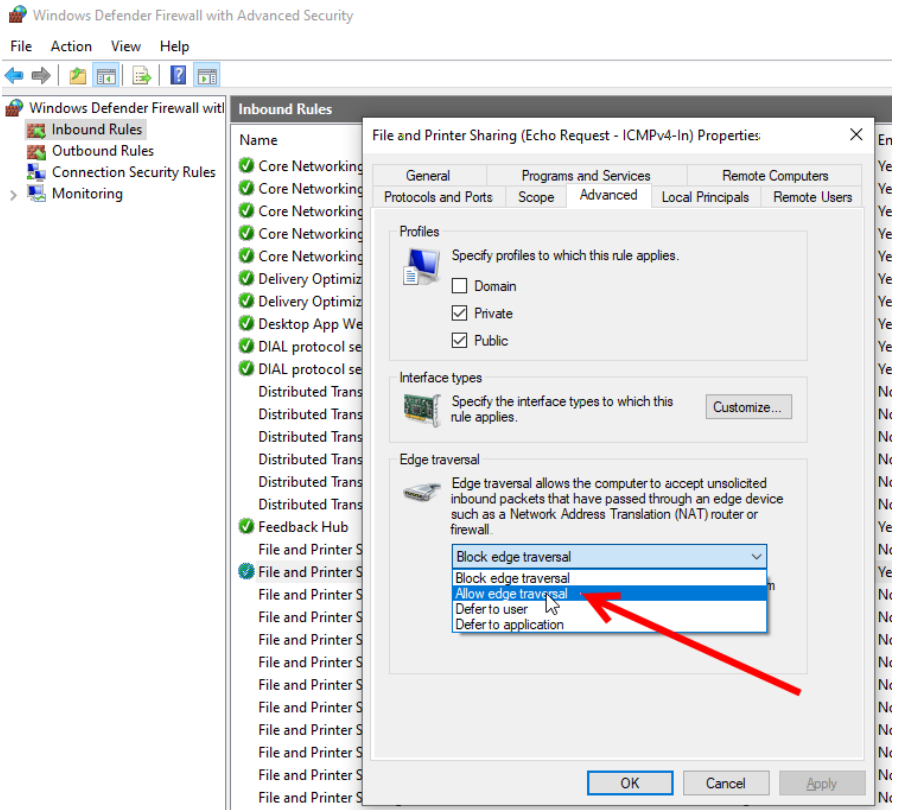
\includegraphics[width=0.85\textwidth]{images/firewall-edge-transversal.PNG}
\end{center}





\item Putty:
\begin{itemize}
    \item Il faut (apparemment) utiliser Putty pour cette manipulation.
    \item Pour communiquer avec le routeur, il faut clicker sur: \textit{serial}, et dans: \textit{Serial line}, écrire: \textit{COM1}\footnote{Si \textit{COM1} ne fonctionne pas, essayer \textit{COM2}, \textit{COM3}, etc. L'ordinateur a plusieurs ports COM, un d'eux sert à communiquer avec le routeur.}.
\end{itemize}





\item Câbles:
\begin{itemize}
    \item câble \textcolor{yellow}{\textbf{jaune}} = internet,
    \item câble \textcolor{green}{\textbf{vert}} = réseau interne,
    \item câble \textcolor{blue}{\textbf{bleu}} = pour la configuration.
\end{itemize}
\textbf{Remarque:} les câbles ne sont \textbf{pas} interchangeables. Si vous utilisez un câble vert au lieu d'un bleu, vous n'arriverez pas à faire la configuration.





\item Câblage:
\begin{enumerate}
    %\item L’interconnexion entre vos 2 routeurs est un câble série (en rouge sur le plan). Regardez bien les connecteurs aux extrémités de ce câble. L’un est de type DTE et l’autre de type DCE. Le DCE est le côté où la clock sera configurée.

    % 1. connecter la console, etc. (puis débrancher)
    % 2. connecter chaque pc à son switch
    % 3. connecter chaque switch à son routeur
    % 4. connecter les routeurs entre eux (!! DTE, DCE !!)


    \item Connecter l'ordinateur au switch pour effacer la configuration:
    \begin{enumerate}
        \item Comme on fait de la configuration, il faut un câble \textcolor{blue}{\textbf{bleu}}. Par exemple, si vous avez le PC 15, il faut aller au panneau de brassage (là où on connecte les câbles) et brancher le câble dans le port 15 \textcolor{blue}{\textbf{bleu}}.
        \item Pour savoir où brancher l'autre extrémité du câble, il faut savoir où se trouve notre switch. Si le switch est à côté du port A2-15, on branche le câble dans ce port.
        \item Maintenant, on utilise un autre câble \textcolor{blue}{\textbf{bleu}} pour connecter le port A2-15 (à côté du switch) au port \textit{console} du switch. \\
        \textbf{Remarque:} le port console du switch se trouve \textit{derrière} le switch.
    \end{enumerate}


    \item Connecter l'ordinateur au routeur pour le configurer:
    \begin{enumerate}
        \item Débrancher le câble \textcolor{blue}{\textbf{bleu}} qui connecte le port A2-15 au switch et le connecter au routeur dans le port \textit{console}.
    \end{enumerate}


    \item Connecter l'ordinateur au routeur pour faire le réseau interne:
    \begin{enumerate}
        \item Débrancher tous les câbles \textcolor{blue}{\textbf{bleus}}.
        \item Brancher un câble \textcolor{green}{vert} qui va du port 15 \textcolor{green}{vert} du panneau de brassage au port A2-15 (sur le même panneau).
        \item Brancher un câble \textcolor{green}{vert} du port A2-15 (à côté du switch) au switch.
        \item Brancher un câble \textcolor{green}{vert} du switch au routeur. \textbf{Attention}, il faut le brancher dans le bon port, celui-ci dépend de la configuration du routeur.
        \item Pour l'interconnexion des routeurs, il faut un câble série. Le côté où il est marqué DCE (pas DTE) doit aller dans le routeur où la clock a été configuré. Ici aussi, il faut faire attention à brancher dans le bon port (\texttt{Serial0} ou \texttt{Serial1}) en fonction de la configuration des routeurs.
    \end{enumerate}


\end{enumerate}





\end{itemize}





\begin{figure}[H]
    \centering
    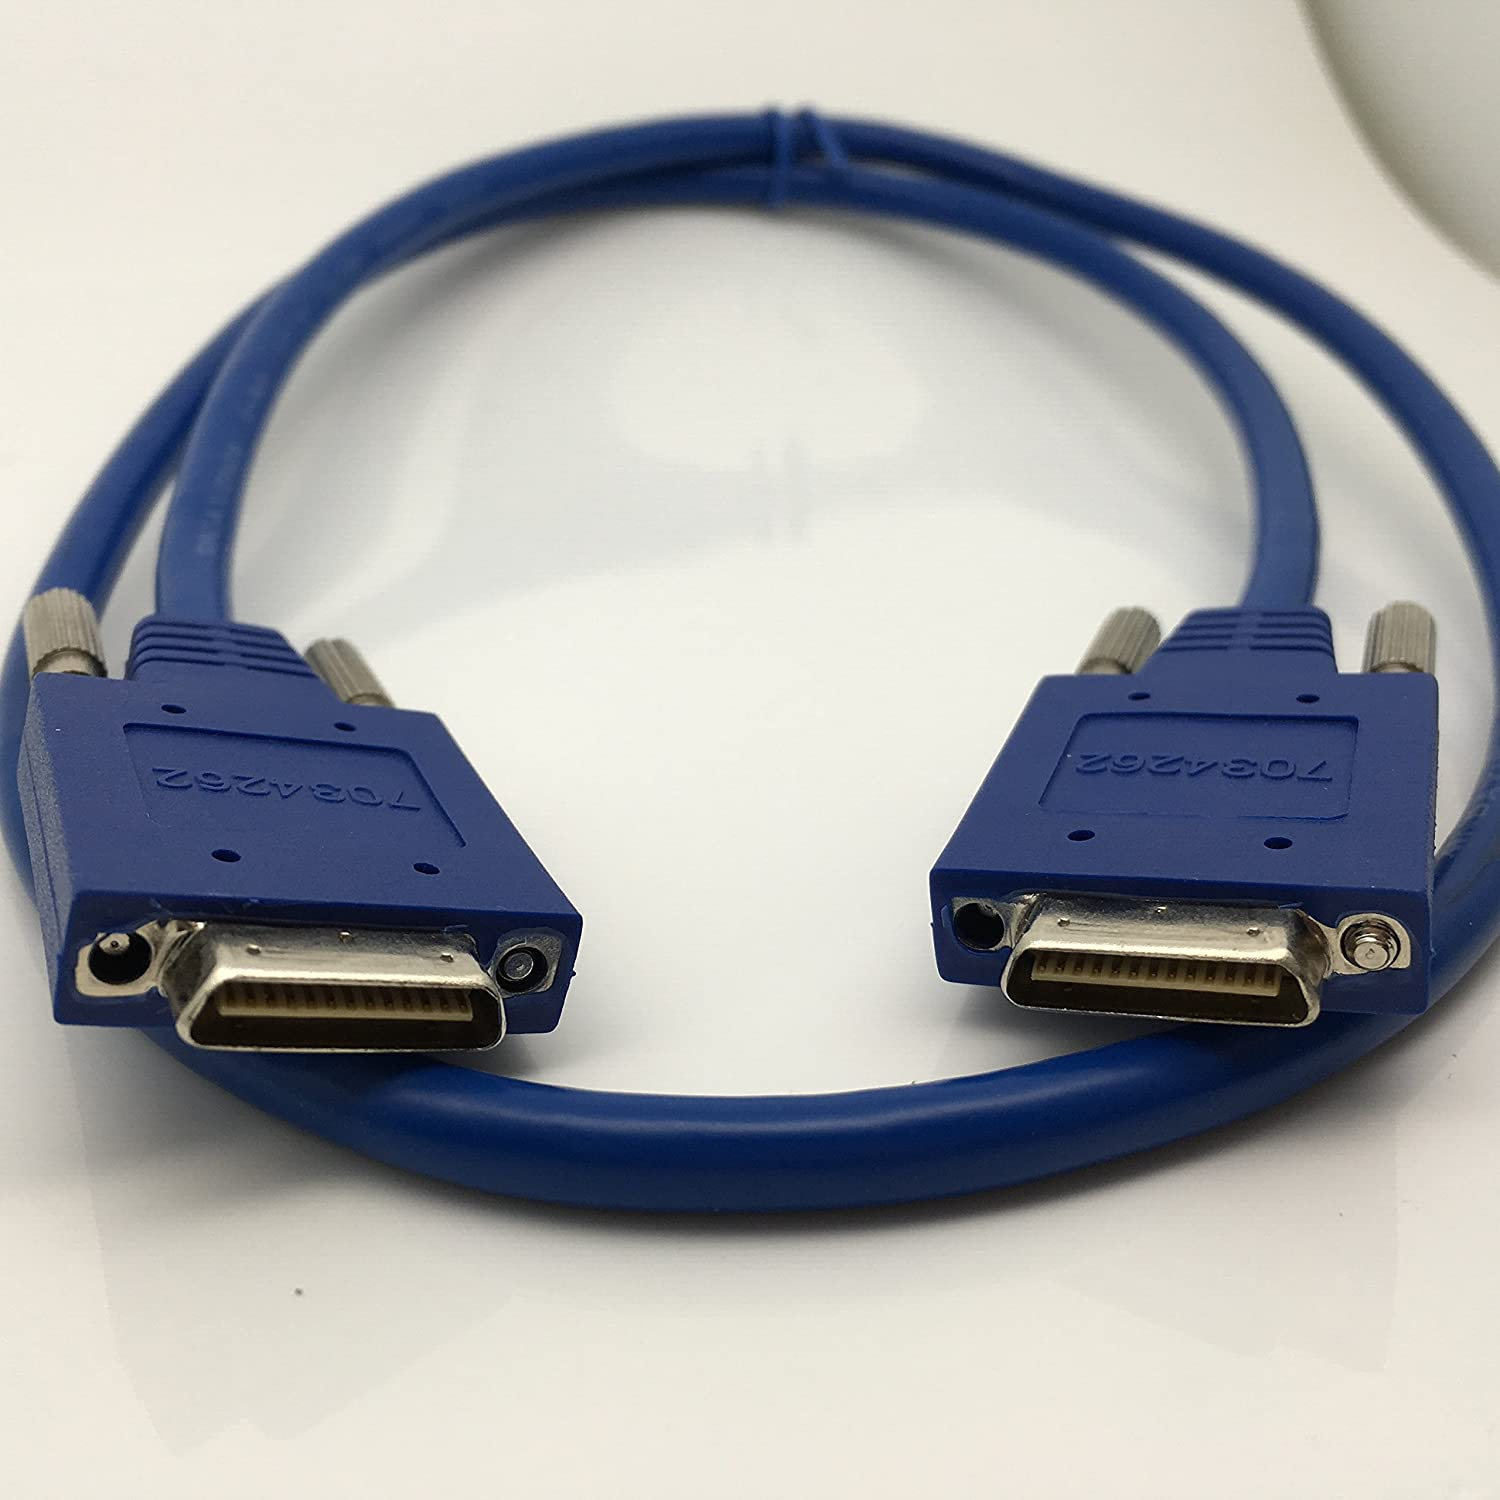
\includegraphics[width=0.70\textwidth]{images/cables-series01.jpg}
    \caption{Câble série}
    \label{fig:cableSerie01}
\end{figure}

\begin{figure}[H]
    \centering
    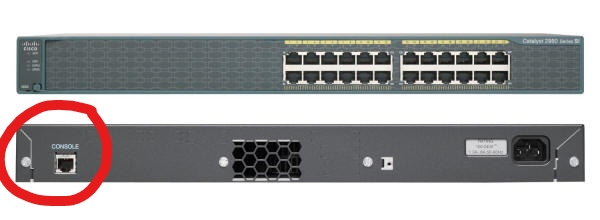
\includegraphics[width=0.85\textwidth]{images/switch02.jpg}
    \caption{Port console switch}
    \label{fig:portConsoleSwitch}
\end{figure}

\begin{figure}[H]
    \centering
    \includegraphics[width=0.98\textwidth]{images/switch-catalyst-2960.jpg}
    \caption{Switch Catalyst 2960}
    \label{fig:switchCatalyst2960}
\end{figure}

\begin{figure}[H]
    \centering
    \includegraphics[width=0.98\textwidth]{images/routeur-cisco-1941.jpg}
    \caption{Routeur Cisco 1941}
    \label{fig:routeurCisco1941}
\end{figure}

\begin{figure}[H]
    \centering
    \includegraphics[width=0.98\textwidth]{images/routeur-cisco-1841.jpg}
    \caption{Routeur Cisco 1841}
    \label{fig:routeurCisco1841}
\end{figure}

\begin{figure}[H]
    \centering
    \includegraphics[width=0.98\textwidth]{images/panneau-brassage01.jpg}
    \caption{Panneau de brassage (1)}
    \label{fig:panneauBrassage01}
\end{figure}

\begin{figure}[H]
    \centering
    \includegraphics[width=0.98\textwidth]{images/panneau-brassage02.jpg}
    \caption{Panneau de brassage (2)}
    \label{fig:panneauBrassage02}
\end{figure}

\begin{figure}[H]
    \centering
    \includegraphics[width=0.98\textwidth]{images/switch-brassage01.jpg}
    \caption{Ports à côté des switchs}
    \label{fig:switchBrassage01}
\end{figure}















\newpage \section{Auto-évaluation (séances 1-4)}





Questions:
\begin{itemize}
    \item Pour passer du mode exec (prompt >) au mode privilege (prompt \#), la commande à entrer est ?
    \begin{example}
        \texttt{enable}
    \end{example}
    \item Pour entrer en mode configuration globale, la commande à entrer est ?
    \begin{example}
        \texttt{configure terminal}
    \end{example}
    \item Pour désactiver les recherches DNS, la commande à exécuter sur le router en mode de configuration est ?
    \begin{example}
        \texttt{no ip domain-lookup}
    \end{example}
    \item Pour encrypter les mots de passe dans le fichier de configuration, la commande à exécuter en mode configuration est ?
    \begin{example}
        \texttt{service password-encryption}
    \end{example}
    \item Pour mettre \textbf{R1} comme hostname sur le router R1, la commande à exécuter en "configuration globale" est ?
    \begin{example}
        \texttt{hostname R1}
    \end{example}
    \item Pour que l'interface g0/0 \textbf{ne soit plus} en état "\texttt{administratively down}", après avoir joué la commande \texttt{interface g0/0}, la commande à exécuter est ?
    \begin{example}
        \texttt{no shutdown}
    \end{example}
    \item Pour mettre la description "vers LAN5" sur l'interface g0/1 sur R2, après avoir joué la commande "\texttt{interface g0/1}", la commande à exécuter est ?
    \begin{example}
        \texttt{description vers LAN5}
    \end{example}
    \item Sur R3, pour configurer l'adresse réseau sur l'interface G0/1, après avoir exécuté "\texttt{interface g0/1}", la commande sera ?
    \begin{example}
        \texttt{ip address <IP> <Netmask x.x.x.x>} \\
        \texttt{ip address 192.168.6.10 255.255.255.0}
    \end{example}
    \item Sur R1, pour configurer l'adresse réseau sur l'interface s0/0/0, après avoir exécuté "\texttt{interface s0/0/0}", la commande sera ?
    \begin{example}
        \texttt{ip address 192.168.7.10 255.255.255.0}
    \end{example}
    \item Sur R1, pour créer une route \textbf{récursive par défaut} afin de pouvoir joindre les différents LAN's, après être entré en mode configuration globale, la commande sera ?
    \begin{example}
        \texttt{ip route <ip\_réseau\_à\_atteindre> <netmask> <ip\_routeur\_qui\_connecte\_aux\_LANs>} \\
        \texttt{ip route 0.0.0.0 0.0.0.0 192.168.7.20}
    \end{example}
    \item Sur R4, pour créer une route \textbf{directement connectée par défaut} afin de pouvoir joindre les différents LAN's, après être entré en mode configuration globale, la commande sera ?
    \begin{example}
        \texttt{ip route <ip\_réseau\_à\_atteindre> <netmask> <interface\_routeur\_à\_atteindre>} \\
        \texttt{ip route 0.0.0.0 0.0.0.0 Serial0/0/0} \\
        \textcolor{red}{\textbf{Attention !}} À l'examen, il vaut mieux mettre l'adresse IP plutôt que l'interface directement. Ça permet d'éviter des problèmes de connexion difficiles à résoudre.
    \end{example}
    \item Sur R2, pour créer une \textbf{route récursive} vers le LAN4, après être entré en mode configuration globale, la commande sera ?
    \begin{example}
        \texttt{ip route 192.168.4.0 255.255.255.0 192.168.8.20}
    \end{example}
    \item Sur R3, pour créer une route \textbf{directement connectée} vers le LAN5, après être entré en mode configuration globale, la commande sera ?
    \begin{example}
        \texttt{ip route 192.168.5.0 255.255.255.0 S0/0/1}
    \end{example}
    \item L'adresse IP à configurer pour le \textbf{default gateway} du PC4 sera ?
    \begin{example}
        \texttt{192.168.4.10}
    \end{example}
\end{itemize}





\begin{figure}[H]
    \centering
    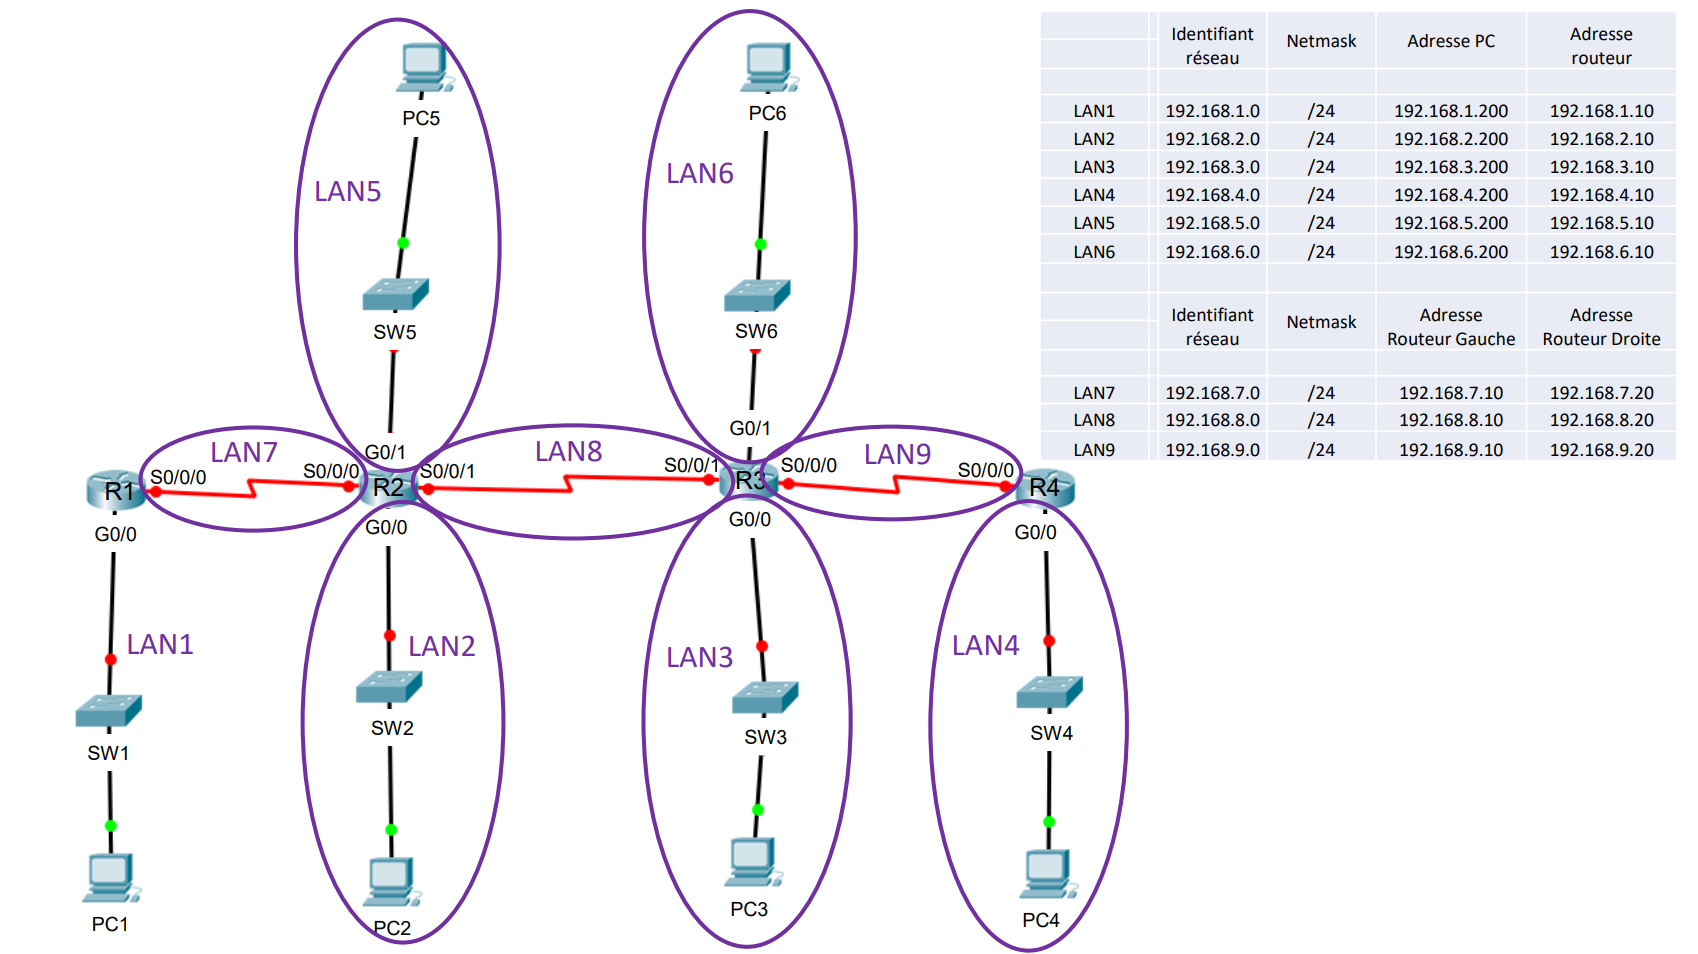
\includegraphics[width=0.98\textwidth]{images/auto-evaluation-1-4-topologie01.PNG}
    \caption{Topologie - auto-évalution - séances 1-4}
    \label{fig:auto-evaluation-1-4-topologie01}
\end{figure}















\newpage \section{Exercice facultatif à réaliser sur Packet Tracer}





\begin{itemize}





\item Topologie:
\begin{center}
    \begin{tikzpicture}
        \node (pc1) [] at (0,0) {
\includegraphics[width=1.5cm]{images/pc.jpg}};
        \node (switch1) [] at (2,-2) {
\includegraphics[width=1.5cm]{images/switch.jpg}};
        \node (router1) [] at (4,0) {
\includegraphics[width=1.5cm]{images/router.jpg}};
        \node (router2) [] at (8,0) {
\includegraphics[width=1.5cm]{images/router.jpg}};
        \node (switch2) [] at (10,-2) {
\includegraphics[width=1.5cm]{images/switch.jpg}};
        \node (pc2) [] at (12,0) {
\includegraphics[width=1.5cm]{images/pc.jpg}};

        \draw [thick, blue] (pc1) -- (switch1);
        \draw [thick, blue] (router1) -- (switch1);
        \draw [thick, red] (router1) -- (router2);
        \draw [thick, green] (switch2) -- (router2);
        \draw [thick, green] (switch2) -- (pc2);

        \node [] at (0,1) {PC-A};
        \node [] at (12,1) {PC-C};
        \node [] at (4,1) {R1};
        \node [] at (8,1) {R3};
        \node [] at (2,-3) {S1};
        \node [] at (10,-3) {S3};

        \node [blue, xshift=-0.5cm] at (switch1.west) {F0/6};
        \node [blue, xshift=0.5cm] at (switch1.east) {F0/5};
        \node [blue, yshift=-0.4cm] at (router1.south) {G0/1};
        \node [red] at (router1.north east) {s0/0/1};
        \node [red] at (router2.north west) {s0/0/0};
        \node [red, xshift=-0.5cm, yshift=0.2cm] at (router2.south west) {DCE};
        \node [red, xshift=0.5cm, yshift=0.2cm] at (router1.south east) {DTE};
        \node [green, xshift=-0.5cm] at (switch2.west) {F0/5};
        \node [green, xshift=0.5cm] at (switch2.east) {F0/18};
        \node [green, yshift=-0.4cm] at (router2.south) {G0/1};
    \end{tikzpicture}
\end{center}





\item Configuration des machines:
\begin{center}
    \begin{tabular}{|c|c|c|c|} \hline
        & IP address & Default gateway \\ \hline
        PC-A & 192.168.0.10/24 & 192.168.0.1/24 \\ \hline
        PC-C & 192.168.1.10/24 & 192.168.1.1/24 \\ \hline
    \end{tabular}
    \\
    \begin{tabular}{|c|c|c|c|} \hline
        & Interface & IP address & Default gateway \\ \hline
        
        \multirow{2}{*}{R1}
        & G0/1 & 192.168.0.1/24 & / \\
        & S0/0/1 & 10.1.1.1/30 & / \\ \hline
        
        \multirow{2}{*}{R3}
        & G0/1 & 192.168.1.1/24 & / \\
        & S0/0/0 & 10.1.1.2/30 & / \\ \hline
    \end{tabular}
\end{center}





\item R3 a aussi des interfaces internes (lo0, lo1 = loopback):
\begin{center}
    \begin{tabular}{|c|c|c|c|} \hline
        & Interface & IP address & Default gateway \\ \hline

        \multirow{2}{*}{R3}
        & Lo0 & 209.165.200.225/27 & / \\
        & Lo1 & 198.133.219.1/24 & / \\ \hline
    \end{tabular}
\end{center}





\item Matériel:
\begin{itemize}
    \item routeur = cisco 1941
    \item switch = cisco 2960
    \item PC, câbles ethernet, câble série, câbles consoles (pour la configuration)
\end{itemize}





\item Pour que les routeurs puissent communiquer entre eux, il faut ajouter des cartes réseau qui servent aux connections séries:
\begin{center}
    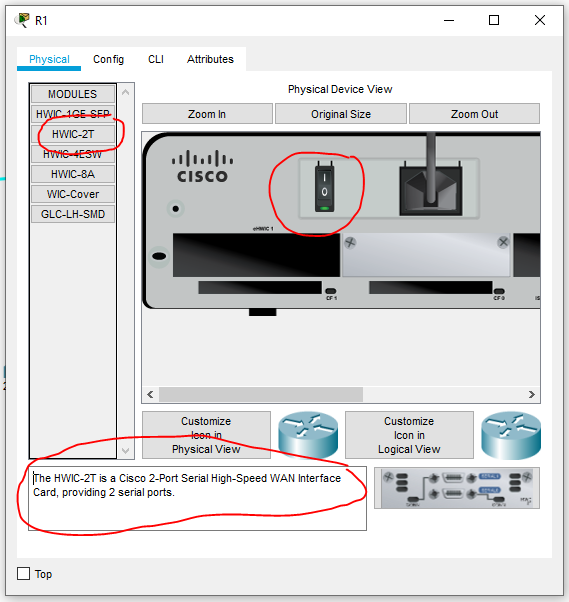
\includegraphics[width=0.45\textwidth]{images/interface-reseau-serie01.PNG}
    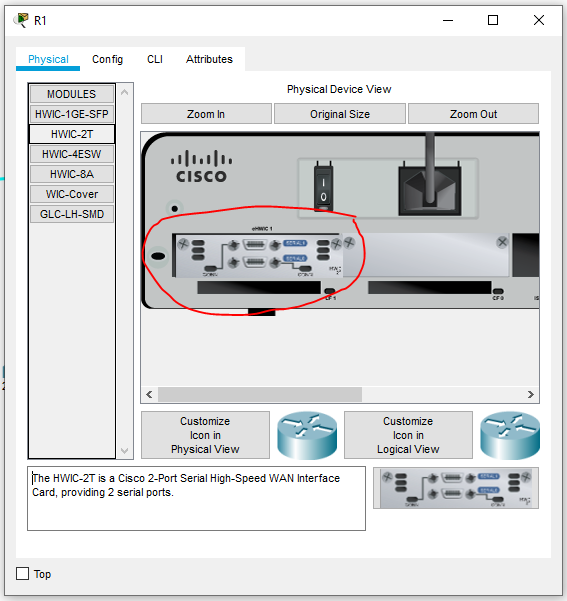
\includegraphics[width=0.45\textwidth]{images/interface-reseau-serie02.PNG}
\end{center}
\textcolor{red}{\textbf{Attention.}} Si on met la carte réseau à gauche, on aura \texttt{s0/1/0} et \texttt{s0/1/1}. Pour avoir les interfaces exactement comme dans l'énoncé, il faut placer la carte réseau à \textit{droite}.





\item Les interfaces Lo0 et Lo1 sont des interfaces de loopback donc il n'y a pas besoin de rajouter un composant physique (à R3).





\end{itemize}










\subsection{Placer les appareils et les initialiser}





\begin{enumerate}



\item Connecter le câble console (\textcolor{cyan}{cyan}) du port RS-232 du PC vers les ports console des switchs.
\item Clicker sur le PC, aller dans l'onglet \textit{Desktop} et clicker sur \textit{Terminal}, puis sur \textit{Ok}.
\item Taper les commandes:
\begin{enumerate}
    \item \texttt{enable}
    \item \texttt{delete flash:vlan.dat}
    \begin{example}
        \textbf{Remarques:}
        \begin{itemize}
            \item Si on ne peut pas le supprimer parce que le fichier \textit{vlan.dat} n'existe pas, c'est un bonne chose vu qu'on veut justement qu'il n'y en ait pas.
            \item On peut mettre \textit{flash:vlan.dat} ou \textit{vlan.dat}.
        \end{itemize}
    \end{example}
    \item \texttt{erase startup-config}
    \item \texttt{reload}
\end{enumerate}



\item Connecter le câble console (\textcolor{cyan}{cyan}) du port RS-232 du PC vers les ports console des routeurs.
\item Clicker sur le PC, aller dans l'onglet \textit{Desktop} et clicker sur \textit{Terminal}, puis sur \textit{Ok}.
\item Taper les commandes:
\begin{enumerate}
    \item \texttt{enable}
    \item \texttt{erase startup-config}
    \item \texttt{reload}
    \begin{example}
        \textbf{Remarque:} quand le terminal propose d'entrer le \textit{dialogue de configuration initiale}, il faut refuser.
    \end{example}
\end{enumerate}



\end{enumerate}










\subsection{Configuration réseau de base des routeurs et des pc}





\begin{enumerate}



\item Clicker sur les PC et aller dans l'onglet \textit{Config}. Dans \textit{Settings}, mettre la gateway et dans \textit{FastEthernet0}, mettre l'adresse ip et le netmask.
\begin{example}
    \textbf{Remarque:} pour vérifier la configuration, on peut aller dans l'onglet \textit{Desktop}, clicker sur \textit{Command Prompt} et taper la commande: \texttt{ipconfig}.
\end{example}



\item Connecter le câble console (\textcolor{cyan}{cyan}) du port RS-232 du PC vers les ports console des routeurs.
\item Clicker sur le PC, aller dans l'onglet \textit{Desktop} et clicker sur \textit{Terminal}, puis sur \textit{Ok}.
\item Pour configurer les routeurs, il y a plusieurs étapes:
\begin{enumerate}
    \item entrer en mode configuration globale
    \begin{itemize}
        \item \texttt{enable}
        \item \texttt{configure terminal}
    \end{itemize}
    \item désactiver les recherches DNS et configurer la console en mode synchrone
    \begin{itemize}
        \item \texttt{no ip domain-lookup}
        \item \texttt{line console 0}
        \item \texttt{logging synchronous}
        \item \texttt{exit}
    \end{itemize}
    \item configurer l'interface \texttt{g0/1} (qui communique avec les pc)
    \begin{itemize}
        \item \texttt{interface g0/1}
        \item \texttt{ip address <IP> <Netmask x.x.x.x>}
        \begin{example}
            \begin{itemize}
                \item R1: ip = \texttt{192.168.0.1} \; ; \; netmask = \texttt{255.255.255.0}
                \item R3: ip = \texttt{192.168.1.1} \; ; \; netmask = \texttt{255.255.255.0}
            \end{itemize}
        \end{example}
        \item \texttt{no shutdown}
        \item \texttt{exit}
    \end{itemize}
    \item configurer l'interface qui communique avec l'autre routeur
    \begin{itemize}
        \item \texttt{interface <interface\_routeur>}
        \begin{example}
            \begin{itemize}
                \item R1: \texttt{s0/0/1}
                \item R1: \texttt{s0/0/0}
            \end{itemize}
        \end{example}
        \item \texttt{ip address <IP> <Netmask x.x.x.x>}
        \begin{example}
            \begin{itemize}
                \item R1: ip = \texttt{10.1.1.1} \; ; \; netmask = \texttt{255.255.255.252}
                \item R3: ip = \texttt{10.1.1.2} \; ; \; netmask = \texttt{255.255.255.252}
            \end{itemize}
        \end{example}
        \item \textbf{Seulement pour R3} (DCE = clock configurée ici): \texttt{clock rate 128000}
        \item \texttt{no shutdown}
        \item \texttt{exit}
    \end{itemize}
    \item \textbf{seulement pour R3}, on configure les interfaces de loopback:
    \begin{itemize}
        \item \texttt{interface Lo0}
        \item \texttt{ip address 209.165.200.225 255.255.255.224}
        \item \texttt{no shutdown}
        \item \texttt{exit}
        \item \texttt{interface Lo1}
        \item \texttt{ip address 198.133.219.1 255.255.255.0}
        \item \texttt{no shutdown}
        \item \texttt{exit}
    \end{itemize}
    \item ajouter les routes sur les routeurs: \texttt{ip route 0.0.0.0 0.0.0.0 <IP\_autre\_routeur>}
    \begin{example}
        \begin{itemize}
            \item R1: ip = \texttt{10.1.1.2}
            \item R3: ip = \texttt{10.1.1.1}
        \end{itemize}
    \end{example}
\end{enumerate}



\end{enumerate}










\subsection{Câblage et vérification}





\begin{enumerate}



    \item Enlever les câbles consoles (\textcolor{cyan}{cyan}).



    \item Connecter les deux routeurs avec un câble série (DCE du côté R3) et connecter les autres appareils avec un câble \textit{Copper Straight Through}.
    \begin{center}
        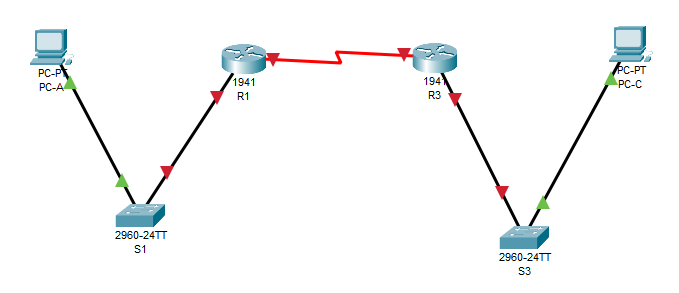
\includegraphics[width=0.75\textwidth]{images/Packet-Tracer-End-Result01.PNG}
    \end{center}



    \item Maintenant qu'on a tout configuré et câblé, on essaie de ping le PC-C avec le PC-A.
    \begin{example}
        \texttt{ping 192.168.1.10}
    \end{example}



\end{enumerate}















\section{Labo 5 --- Calcul des sous-réseaux}





\begin{itemize}





\item Topologie:
\begin{center}
    \begin{tikzpicture}

        \node (pc1) [] at (0,0) {
\includegraphics[width=1.5cm]{images/pc.jpg}};
        \node (switch1) [] at (4,0) {
\includegraphics[width=1.5cm]{images/switch.jpg}};
        \node (router1) [] at (8,0) {
\includegraphics[width=1.5cm]{images/router.jpg}};
        \node (pc2) [] at (12,0) {
\includegraphics[width=1.5cm]{images/pc.jpg}};

        \draw [thick, blue] (pc1) -- (switch1);
        \draw [thick, blue] (router1) -- (switch1);
        \draw [thick, red] (router1) -- (pc2);

        \node [] at (0,1) {PC-A};
        \node [] at (4,1) {S1};
        \node [] at (8,1) {R1};
        \node [] at (12,1) {PC-B};

        \node [blue, yshift=0.5cm, xshift=-0.5cm] at (switch1.west) {F0/6};
        \node [blue, yshift=0.5cm, xshift=+0.5cm] at (switch1.east) {F0/5};
        \node [blue, yshift=0.5cm, xshift=-0.5cm] at (router1.west) {G0/1};
        \node [red,  yshift=0.5cm, xshift=+0.5cm] at (router1.east) {G0/0};

    \end{tikzpicture}
\end{center}




\item Matériel:
\begin{itemize}
    \item routeur = cisco 1941
    \item switch = cisco 2960
    \item PC, câbles ethernet, câbles consoles (pour la configuration)
\end{itemize}





\end{itemize}










\subsection{Attribution des adresses ip}





\begin{itemize}





\item Situation:
\begin{itemize}
    \item réseau = 192.168.0.0/24,
    \item 1er sous-réseau = 25 ip,
    \item 2ème sous-réseau = 10 ip,
    \item 3 et 4èmes sous-réseaux (lo0 et lo1) = sous-réseaux réservés
    \item 5 et 6èmes sous-réseaux = sous-réseaux réservés
\end{itemize}
\textbf{Remarque:} tous les sous-réseaux doivent être de même taille.





\item 6 sous-réseaux $ \implies $ 3 bits de sous-réseau \& 5 bits d'adressage $ \implies 2^5 = 32 $ adresses.
\begin{itemize}
    \item 1er sous-réseau = 192.168.0000 0000.0/27 = 192.168.0.0/27
    \item 2ème sous-réseau = 192.168.0010 0000.0/27 = 192.168.32.0/27
    \item 3ème sous-réseau = 192.168.0100 0000.0/27 = 192.168.64.0/27
    \item 4ème sous-réseau = 192.168.0110 0000.0/27 = 192.168.96.0/27
    \item 5ème sous-réseau = 192.168.1000 0000.0/27 = 192.168.128.0/27
    \item 6ème sous-réseau = 192.168.1010 0000.0/27 = 192.168.160.0/27
    \item netmask = 255.255.255.224
\end{itemize}





\item Configuration des machines:
\begin{center}
    \begin{tabular}{|c|c|c|c|} \hline
        & IP address & Default gateway \\ \hline
        PC-A & 192.168.0.2/27 & 192.168.0.1 \\ \hline
        PC-B & 192.168.32.2/27 & 192.168.32.1 \\ \hline
    \end{tabular}
    \\
    \begin{tabular}{|c|c|c|c|} \hline
        & Interface & IP address & Default gateway \\ \hline

        \multirow{4}{*}{R1}
        & G0/0 & 192.168.32.1/27 & / \\
        & G0/1 & 192.168.0.1/27 & / \\

        & Lo0 & 192.168.64.1/27 & / \\
        & Lo1 & 192.168.96.1/27 & / \\ \hline
    \end{tabular}
\end{center}





\end{itemize}










\subsection{Configuration des machines}





\begin{enumerate}





\item Clicker sur les PC et aller dans l'onglet \textit{Config}. Dans \textit{Settings}, mettre la gateway et dans \textit{FastEthernet0}, mettre l'adresse ip et le netmask.
\begin{example}
    \textbf{Remarque:} pour vérifier la configuration, on peut aller dans l'onglet \textit{Desktop}, clicker sur \textit{Command Prompt} et taper la commande: \texttt{ipconfig}.
\end{example}





\item Initialiser le switch:
\begin{enumerate}
    \item connecter le câble console (\textcolor{cyan}{cyan}) du port RS-232 du PC au port console du switch,
    \item clicker sur le PC, aller dans l'onglet \textit{Desktop}, clicker sur \textit{Terminal}, puis sur \textit{Ok},
    \item entrer les commandes suivantes:
    \begin{itemize}
        \item \texttt{enable}
        \item \texttt{delete vlan.dat}, ou: \texttt{delete flash:vlan.dat}
        \item \texttt{erase startup-config}
        \item \texttt{reload}
    \end{itemize}
\end{enumerate}





\item Configurer le routeur:
\begin{enumerate}
    \item connecter le câble console (\textcolor{cyan}{cyan}) du port RS-232 du PC au port console du routeur,
    \item clicker sur le PC, aller dans l'onglet \textit{Desktop}, clicker sur \textit{Terminal}, puis sur \textit{Ok},
    \item initialiser le routeur:
    \begin{itemize}
        \item \texttt{enable}
        \item \texttt{erase startup-config}
        \item \texttt{reload}
        \begin{example}
            \textbf{Remarque:} refuser d'entrer dans le \textit{dialogue de configuration initiale}.
        \end{example}
    \end{itemize}
    \item entrer en mode configuration globale:
    \begin{itemize}
        \item \texttt{enable}
        \item \texttt{configure terminal}
    \end{itemize}
    \item désactiver les recherches dns et configurer la console en mode synchrone:
    \begin{itemize}
        \item \texttt{no ip domain-lookup}
        \item \texttt{line console 0}
        \item \texttt{logging synchronous}
        \item \texttt{exit}
    \end{itemize}
    \item configurer les interfaces:
    \begin{itemize}
        \item \texttt{interface <interface>}
        \begin{example}
            g0/0, g0/1, lo0, lo1
        \end{example}
        \item \texttt{ip address <ip> <netmask>}
        \begin{example}
            \begin{itemize}
                \item g0/0: ip = 192.168.32.1, netmask = 255.255.255.224
                \item g0/1: ip = 192.168.0.1, netmask = 255.255.255.224
                \item lo0: ip = 192.168.64.1, netmask = 255.255.255.224
                \item lo1: ip = 192.168.96.1, netmask = 255.255.255.224
            \end{itemize}
        \end{example}
        \item \texttt{no shutdown}
        \item \texttt{exit}
    \end{itemize}
\end{enumerate}





\end{enumerate}















\newpage \section{Auto-évalutation (séance 5)}





\begin{itemize}





\item Réseau à diviser en sous-réseaux: 172.16.52.128/25.





\item 6 sous-réseaux $ \implies $ 3 bits de sous-réseau \& 4 bits d'adressage $ \implies 2^4 = 16 $ adresses.
\begin{itemize}
    \item 1er sous-réseau = 172.16.52.1000 0000/28 = 172.16.52.128/28
    \item 2ème sous-réseau = 172.16.52.1001 0000/28 = 172.16.52.144/28
    \item 3ème sous-réseau = 172.16.52.1010 0000/28 = 172.16.52.160/28
    \item 4ème sous-réseau = 172.16.52.1011 0000/28 = 172.16.52.176/28
    \item 5ème sous-réseau = 172.16.52.1100 0000/28 = 172.16.52.192/28
    \item 6ème sous-réseau = 172.16.52.1101 0000/28 = 172.16.52.208/28
    \item netmask = 255.255.255.240
\end{itemize}





\item Configuration des machines:
\begin{center}
    \begin{tabular}{|c|c|c|c|c|} \hline
        & & IP address & Netmask & Default Gateway \\ \hline

        \multirow{3}{*}{\textbf{LAN1}}
        & Router1 & 172.16.52.142 & 255.255.255.240 & / \\
        & Laptop1 & 172.16.52.129 & 255.255.255.240 & 172.16.52.142 \\
        & Laptop2 & 172.16.52.130 & 255.255.255.240 & 172.16.52.142 \\ \hline

        \multirow{2}{*}{\textbf{LAN2}}
        & Router2 & 172.16.52.158 & 255.255.255.240 & / \\
        & PC1 & 172.16.52.145 & 255.255.255.240 & 172.16.52.158 \\ \hline

        \multirow{2}{*}{\textbf{LAN3}}
        & Router3 & 172.16.52.174 & 255.255.255.240 & / \\
        & Laptop3 & 172.16.52.163 & 255.255.255.240 & 172.16.52.174 \\ \hline

        \multirow{2}{*}{\textbf{LAN4}}
        & Router3 & 172.16.52.190 & 255.255.255.240 & / \\
        & Server1 & 172.16.52.177 & 255.255.255.240 & 172.16.52.190 \\ \hline

        \multirow{2}{*}{\textbf{LAN5}}
        & Router1 & 172.16.52.193 & 255.255.255.240 & / \\
        & Router3 & 172.16.52.206 & 255.255.255.240 & / \\ \hline

        \multirow{2}{*}{\textbf{LAN6}}
        & Router2 & 172.16.52.222 & 255.255.255.240 & / \\
        & Router3 & 172.16.52.209 & 255.255.255.240 & / \\ \hline
    \end{tabular}
\end{center}





\end{itemize}





\begin{figure}[H]
    \centering
    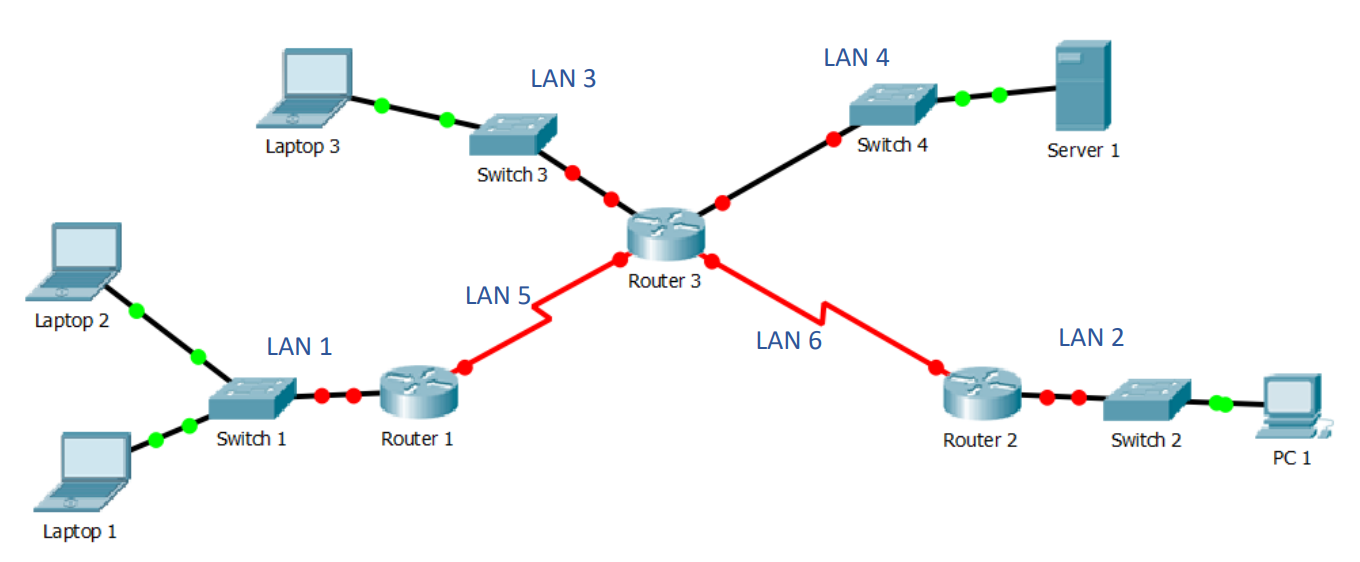
\includegraphics[width=0.95\textwidth]{images/auto-evaluation-5-topologie01.PNG}
    \caption{Topologie - auto-évaluation - séance 5}
    \label{fig:topologieAutoEvaluationSeance5}
\end{figure}





Questions:
\begin{itemize}
    \item Quel masque de sous-réseau vont avoir vos LAN's? exprimez le sous forme xxx.xxx.xxx.xxx
    \begin{example}
        255.255.255.240
    \end{example}
    \item LAN 1: Quelle sera l'adresse IP du Router1 sur le LAN1?
    \begin{example}
        172.16.52.142
    \end{example}
    \item LAN 1: Quelle sera l'adresse IP et netmask du Laptop1 (par exemple: 192.168.1.10/27)?
    \begin{example}
        172.16.52.129/28
    \end{example}
    \item LAN 1: Quelle sera Le default gateway du Laptop1?
    \begin{example}
        172.16.52.142
    \end{example}
    \item LAN 1: Quelle sera l'adresse IP et netmask du Laptop2 (par exemple: 192.168.1.10/27)?
    \begin{example}
        172.16.52.130/28
    \end{example}
    \item LAN 1: Quelle sera Le default gateway du Laptop2?
    \begin{example}
        172.16.52.142
    \end{example}
    \item LAN 2: Quelle sera l'adresse IP du Router2 sur le LAN2?
    \begin{example}
        172.16.52.158
    \end{example}
    \item LAN 2: Quelle sera l'adresse IP et netmask du PC1 (par exemple: 192.168.1.10/27)?
    \begin{example}
        172.16.52.145/28
    \end{example}
    \item LAN 2: Quelle sera Le default gateway du PC1?
    \begin{example}
        172.16.52.158
    \end{example}
    \item LAN 3: Quelle sera l'adresse IP du Router3 sur le LAN3?
    \begin{example}
        172.16.52.174
    \end{example}
    \item LAN 3: Quelle sera l'adresse IP et netmask du Laptop3 (par exemple: 192.168.1.10/27)?
    \begin{example}
        172.16.52.163/28
    \end{example}
    \item LAN 3: Quelle sera Le default gateway du PC1? \\
    \textcolor{red}{\textbf{Attention !}} la vraie question est: \textit{quelle est la default gateway du Laptop 3 ?}
    \begin{example}
        172.16.52.174
    \end{example}
    \item LAN 4: Quelle sera l'adresse IP du Router3 sur le LAN4?
    \begin{example}
        172.16.52.190
    \end{example}
    \item LAN 4: Quelle sera l'adresse IP et netmask du Server1 (par exemple: 192.168.1.10/27)?
    \begin{example}
        172.16.52.177/28
    \end{example}
    \item LAN 4: Quelle sera Le default gateway du Server1?
    \begin{example}
        172.16.52.190
    \end{example}
    \item LAN 5: Quelle sera l'adresse IP du Router1 sur le LAN5?
    \begin{example}
        172.16.52.193
    \end{example}
    \item LAN 5: Quelle sera l'adresse IP du Router3 sur le LAN5?
    \begin{example}
        172.16.52.206
    \end{example}
    \item LAN 6: Quelle sera l'adresse IP du Router2 sur le LAN6?
    \begin{example}
        172.16.52.222
    \end{example}
    \item LAN 6: Quelle sera l'adresse IP du Router3 sur le LAN6?
    \begin{example}
        172.16.52.209
    \end{example}
\end{itemize}















\section{Labo 6 --- Accès SSH \& Sécurisation d'équipement}










\subsection{Préparations}





\begin{itemize}





\item Objectif = configurer les machines pour qu'elles acceptent les sessions SSH pour la gestion à distance.





\item Topologie:
\begin{center}
    \begin{tikzpicture}

        \node (router1) [] at (0,0) {
\includegraphics[width=1.5cm]{images/router.jpg}};
        \node (switch1) [] at (5,0) {
\includegraphics[width=1.5cm]{images/switch.jpg}};
        \node (pc1) [] at (10,0) {
\includegraphics[width=1.5cm]{images/pc.jpg}};

        \draw [thick, blue] (router1) -- (switch1);
        \draw [thick, blue] (pc1) -- (switch1);

        \node [] at (0,1) {R1};
        \node [] at (5,1) {S1};
        \node [] at (10,1) {PC-A};

        \node [blue, yshift=0.5cm, xshift=0.5cm] at (router1.east) {G0/1};
        \node [blue, yshift=0.5cm, xshift=-0.5cm] at (switch1.west) {F0/5};
        \node [blue, yshift=0.5cm, xshift=+0.5cm] at (switch1.east) {F0/6};

    \end{tikzpicture}
\end{center}





\item Configuration des machines:
\begin{center}
    \begin{tabular}{|c|c|c|c|} \hline
        & IP address & Netmask & Default Gateway \\ \hline
        R1 -- g0/1 & 192.168.1.1 & 255.255.255.0 & / \\ \hline
        S1 -- vlan1 & 192.168.1.11 & 255.255.255.0 & 192.168.1.1 \\ \hline
        PC-A & 192.168.1.3 & 255.255.255.0 & 192.168.1.1 \\ \hline
    \end{tabular}
\end{center}




\item Matériel:
\begin{itemize}
    \item routeur = cisco 1941
    \item switch = cisco 2960
    \item PC, câbles ethernet, câbles consoles (pour la configuration)
\end{itemize}





\end{itemize}










\subsection{Manipulation}





\begin{enumerate}

    \item Configurer le PC.

    \item Configurer le routeur:
    \begin{enumerate}
        \item initialiser le routeur,
        \item entrer en mode configuration globale,
        \item désactiver les recherches dns et configurer la console en mode synchrone,
        \item configurer l'interface g0/1.
    \end{enumerate}

    \item Initialiser le switch.

    \item Configurer des mesures de sécurité de base sur le routeur:
    \begin{enumerate}
        \item chiffrer les mots de passe: \texttt{service password-encryption},
        \item exiger min 10 caractères pour les mdp: \texttt{security passwords min-length 10},
        \item changer de mdp: \texttt{enable secret <mdp>}.
    \end{enumerate}
    \textbf{Remarque:} le mot de passe sert à passer en mode priviligié (on passe en mode priviligié avec: \texttt{enable}).

    \item Activer la connection SSH sur le routeur:
    \begin{enumerate}
        \item ajouter un nom de domaine: \texttt{ip domain-name CCNA-lab.com},
        \item créer un utilisateur pour la connection en SSH: \texttt{username SSHadmin privilege 1 secret Admin1p@55},
        \item configurer l'entrée des lignes VTY pour autoriser les connexions SSH: \texttt{line vty 0 4},
        \item autoriser uniquement ssh (refuse telnet): \texttt{transport input ssh},
        \item la connection doit se faire sur un compte local: \texttt{login local},
        \item \texttt{exit},
        \item générer une clé avec un modulos de 1024 bits: \texttt{crypto key generate rsa modulus 1024}.
    \end{enumerate}

    \item Sécuriser la console et les lignes VTY sur le routeur:
    \begin{enumerate}
        \item déconnexion après 5 minutes d'inactivité:
        \begin{itemize}
            \item \texttt{line console 0},
            \item \texttt{exec-timeout 5 0},
            \item \texttt{line vty 0 4},
            \item \texttt{exec-timeout 5 0},
            \item \texttt{exit}.
        \end{itemize}
        \item bloquer l'identification pendant 30s après 2 échecs en 2min: \texttt{login block-for 30 attempts 2 within 120}.
    \end{enumerate}

    \item Commandes à utiliser sur le switch:
    \begin{itemize}
        \item \texttt{service password-encryption}
        \item \texttt{enable secret Enablep@55}
        \item \texttt{ip domain-name CCNA-lab.com}
        \item \texttt{username SSHadmin privilege 1 secret Admin1p@55}
        \item \texttt{line vty 0 15}
        \item \texttt{transport input ssh}
        \item \texttt{login local}
        \item \texttt{exit}
        \item \texttt{crypto key generate rsa modulus 1024}
        \item \texttt{line console 0}
        \item \texttt{exec-timeout 10 0}
        \item \texttt{line vty 0 15}
        \item \texttt{exec-timeout 10 0}
        \item \texttt{exit}
        \item \texttt{login block-for 30 attempts 2 within 120}
        \item \texttt{end}
    \end{itemize}

\end{enumerate}










\newpage \subsection{Commandes à utiliser}





\begin{itemize}





\item Routeur:
\begin{verbatim}
enable
erase startup-config
reload

enable
configure terminal

no ip domain-lookup
line console 0
    logging synchronous
exit

interface <interface>                           // ex: g0/1
    ip address <ip> <netmask>                   // ex: 192.168.1.1, 255.255.255.0
    no shutdown
exit

service password-encryption
security passwords min-length 10
enable secret <mdp>                             // ex: 9876543210

ip domain-name <domaine>                        // ex: greg.com
username <username> privilege 1 secret <mdp>    // ex: admin-ssh, 9876543210
line vty 0 4
    transport input ssh
    login local
exit
crypto key generate rsa modulus 1024
    // /!\ erreur /!\
    // hostname <nom_routeur>                   // ex: R1
    // crypto key generate rsa                  // ex. "modulus" = 1024

line console 0
    exec-timeout 5 0
    line vty 0 4
        exec-timeout 5 0
    exit
    login block-for 30 attempts 2 within 120
\end{verbatim}





\newpage \item Switch:
\begin{verbatim}
enable
delete vlan.dat
erase startup-config
reload

enable
configure terminal

interface <interface>                           // ex: vlan1
    ip address <ip> <netmask>                   // ex: 192.168.1.11, 255.255.255.0
    no shutdown
exit
ip default-gateway <gateway>                    // ex: 192.168.1.1

service password-encryption
enable secret <mdp>                             // ex: 9876543210
ip domain-name <domaine>                        // ex: greg.com
username <username> privilege 1 secret <mdp>    // ex: admin-ssh, 9876543210

line vty 0 15
    transport input ssh
    login local
exit
crypto key generate rsa modulus 1024
    // /!\ erreur /!\
    // hostname <nom_routeur>                   // ex: S1
    // crypto key generate rsa                  // ex. "modulus" = 1024

line console 0
    exec-timeout 10 0
    line vty 0 15
        exec-timeout 10 0
    exit
    login block-for 30 attempts 2 within 120
end
\end{verbatim}




\end{itemize}





\begin{figure}[H]
    \centering
    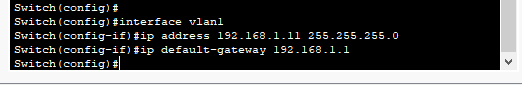
\includegraphics[width=0.75\textwidth]{images/gateway-outside-interface.PNG}
    \caption{(!!!) la commande a changé l'environnement (!!!)}
    \label{}
\end{figure}

\begin{figure}[H]
    \centering
    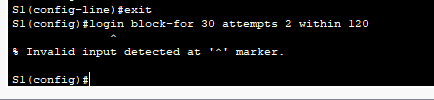
\includegraphics[width=0.75\textwidth]{images/probleme-securite-login01.PNG}
    \caption{Erreur dernière commande switch...}
    \label{}
\end{figure}

\begin{figure}[H]
    \centering
    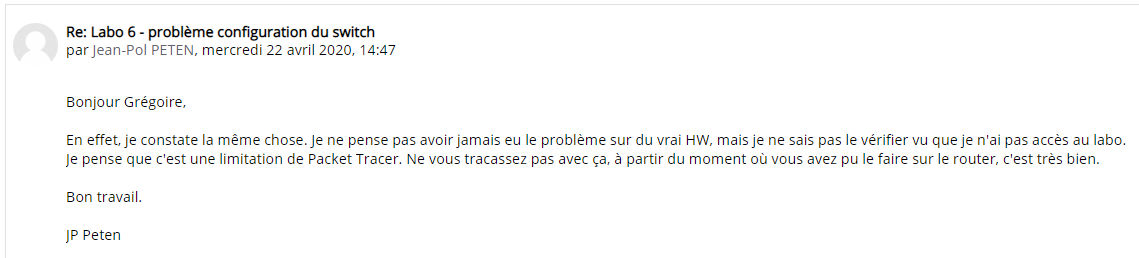
\includegraphics[width=0.95\textwidth]{images/labo6-probleme-securisation-2.PNG}
    \caption{Réponse de JP Peten pour la dernière commande}
    \label{}
\end{figure}










\subsection{Vérifier la bonne implémentation des mesures de sécurité}





\begin{itemize}




\item 





\end{itemize}
















\section{Labo 7 --- VLSM: design et implémentation}










\subsection{Préparation}





\begin{itemize}





\item Topologie:
\begin{center}
    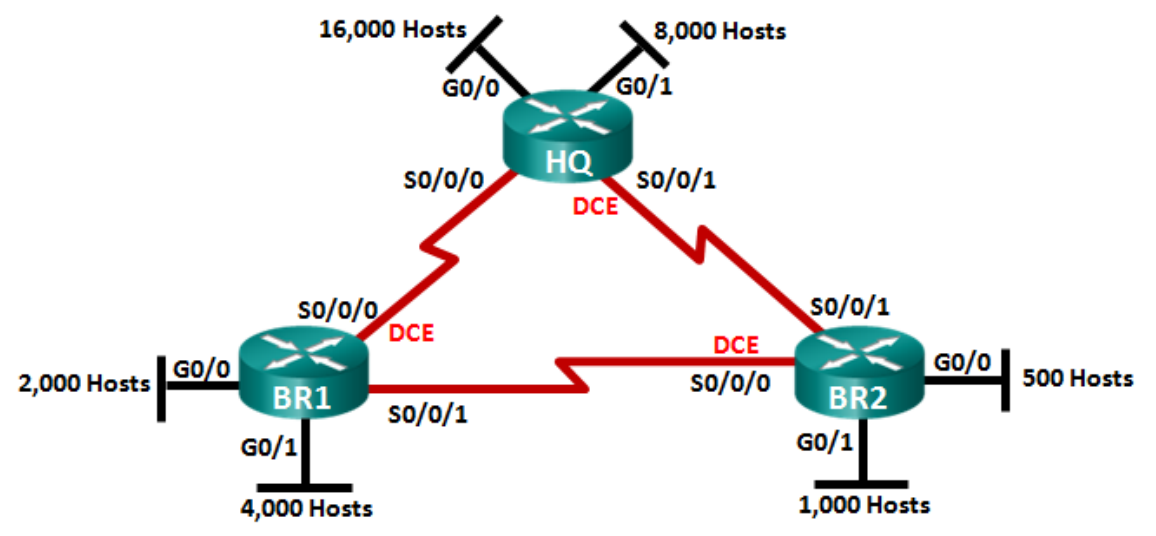
\includegraphics[width=0.85\textwidth]{images/topologie-labo7-01.PNG}
\end{center}





\item Réseau = 172.16.128.0/17





\item Routeur = Cisco 1941





\item Descriptions des sous-réseaux:
\begin{center}
    \begin{tabular}{|c|c|c|c|c|c|} \hline
        & réseau & nb hôtes & netmask & adresse \\ \hline

        \multirow{4}{*}{HQ}
        & \multirow{2}{*}{G0/0} & \multirow{2}{*}{16000}
        & 255.255.1100 0000.0 & 172.16.1000 0000.0 \\
        &&& 255.255.192.0 & 172.16.128.0 \\
        & \multirow{2}{*}{G0/1} & \multirow{2}{*}{8000}
        & 255.255.1110 0000.0 & 172.16.1100 0000.0 \\
        &&& 255.255.224.0 & 172.16.192.0 \\ \hline

        \multirow{4}{*}{BR1}
        & \multirow{2}{*}{G0/1} & \multirow{2}{*}{4000}
        & 255.255.1111 0000.0 & 172.16.1110 0000.0 \\
        &&& 255.255.240.0 & 172.16.224.0 \\
        & \multirow{2}{*}{G0/0} & \multirow{2}{*}{2000}
        & 255.255.1111 1000.0 & 172.16.1111 0000.0 \\ 
        &&& 255.255.248.0 & 172.16.240.0 \\ \hline

        \multirow{4}{*}{BR2}
        & \multirow{2}{*}{G0/1} & \multirow{2}{*}{1000}
        & 255.255.1111 1100.0 & 172.16.1111 1000.0 \\
        &&& 255.255.252.0 & 172.16.248.0 \\
        & \multirow{2}{*}{G0/0} & \multirow{2}{*}{500}
        & 255.255.1111 1110.0 & 172.16.1111 1100.0 \\
        &&& 255.255.254.0 & 172.16.252.0 \\ \hline

        & \multirow{2}{*}{HQ-BR1} & \multirow{2}{*}{2}
        & 255.255.255.1111 1100 & 172.16.254.0000 0000 \\
        &&& 255.255.255.252 & 172.16.254.0 \\ \hline

        & \multirow{2}{*}{HQ-BR2} & \multirow{2}{*}{2}
        & 255.255.255.1111 1100 & 172.16.254.0000 0100 \\
        &&& 255.255.255.252 & 172.16.254.4 \\ \hline

        & \multirow{2}{*}{BR1-BR2} & \multirow{2}{*}{2}
        & 255.255.255.1111 1100 & 172.16.254.0000 1000 \\
        &&& 255.255.255.252 & 172.16.254.8 \\ \hline
    \end{tabular}
\end{center}
\textbf{Remarque:} passage de BR2-G0/0 à HQ-BR1 à HQ-BR2,
\begin{center}
    \begin{tabular}{ll}
        première adresse BR2-G0/0 & 172.16.1111 11\textcolor{red}{\textbf{0}}0 . 0000 0000 \\
        dernière adresse BR2-G0/0 & 172.16.1111 11\textcolor{red}{\textbf{0}}1 . 1111 1111 \\
        première adresse HQ-BR1 &   172.16.1111 11\textcolor{red}{\textbf{1}}0 . 0000 0\textcolor{red}{\textbf{000}} \\
        denrière adresse HQ-BR1 &   172.16.1111 11\textcolor{red}{\textbf{1}}0 . 0000 0\textcolor{red}{\textbf{011}} \\
        première adresse HQ-BR2 &   172.16.1111 11\textcolor{red}{\textbf{1}}0 . 0000 0\textcolor{red}{\textbf{100}} \\
        denrière adresse HQ-BR2 &   172.16.1111 11\textcolor{red}{\textbf{1}}0 . 0000 0\textcolor{red}{\textbf{111}} \\
    \end{tabular}
\end{center}





\item Configuration des interfaces réseaux:
\begin{center}
    \begin{tabular}{|c|c|c|c|} \hline
        appareil & interface & netmask & adresse \\ \hline

        \multirow{4}{*}{HQ}
        & G0/0 & 255.255.192.0 & 172.16.128.1 \\
        & G0/1 & 255.255.224.0 & 172.16.192.1 \\
        & S0/0/0 & 255.255.255.252 & 172.16.254.1 \\
        & S0/0/1 & 255.255.255.252 & 172.16.254.5 \\ \hline

        \multirow{4}{*}{BR1}
        & G0/0 & 255.255.248.0 & 172.16.240.1 \\
        & G0/1 & 255.255.240.0 & 172.16.224.1 \\
        & S0/0/0 & 255.255.255.252 & 172.16.254.2 \\
        & S0/0/1 & 255.255.255.252 & 172.16.254.9 \\ \hline

        \multirow{4}{*}{BR2}
        & G0/0 & 255.255.254.0 & 172.16.252.1 \\
        & G0/1 & 255.255.252.0 & 172.16.248.1 \\
        & S0/0/0 & 255.255.255.252 & 172.16.254.10 \\
        & S0/0/1 & 255.255.255.252 & 172.16.254.6 \\ \hline
    \end{tabular}
\end{center}





\end{itemize}










\subsection{Manipulation}





\begin{itemize}





\item Étape 1: câbler le réseau.
\begin{center}
    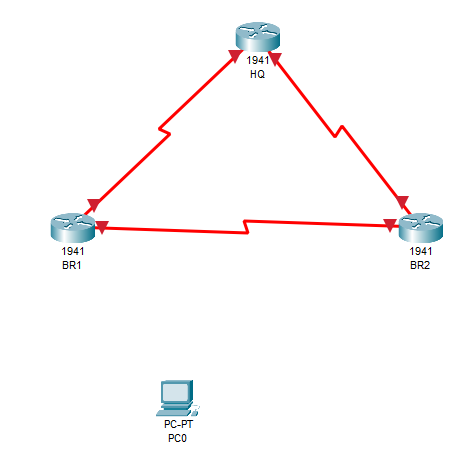
\includegraphics[width=0.65\textwidth]{images/cablage001.PNG}
\end{center}





\item Étape 2: configurer les paramètres de base sur chaque routeur.
\begin{enumerate}
    \item Attribuer le nom de l'appareil au routeur.
    \begin{example}
        \begin{itemize}
            \item \texttt{hostname <nom>}
        \end{itemize}
    \end{example}
    \item Désactiver la recherche DNS pour empêcher le routeur de tenter de traduire des commandes entrées incorrectement comme s'il s'agissait de noms d'hôtes.
    \begin{example}
        \begin{itemize}
            \item \texttt{enable}
            \item \texttt{configure terminal}
            \item \texttt{no ip domain-lookup}
        \end{itemize}
    \end{example}
    \item Attribuer "class" comme mot de passe chiffré EXEC privilégié.
    \begin{example}
        \begin{itemize}
            \item \texttt{enable secret <mdp>}
        \end{itemize}
    \end{example}
    \item Attribuer "cisco" comme mot de passe de la console et activer la connexion.
    \begin{example}
        \begin{itemize}
            \item \texttt{line console 0}
            \item \texttt{password <mdp>}
            \item \texttt{login}
        \end{itemize}
    \end{example}
    \item Attribuer "cisco" comme mot de passe VTY et activer la connexion.
    \begin{example}
        \begin{itemize}
            \item \texttt{line vty 0 4}
            \item \texttt{password <mdp>}
            \item \texttt{login local}
        \end{itemize}
    \end{example}
    \item Chiffrer les mots de passe en texte clair.
    \begin{example}
        \begin{itemize}
            \item \texttt{service password-encryption}
        \end{itemize}
    \end{example}
    \item Créer une bannière qui avertira toute personne accédant à l'appareil qu'un accès non autorisé est interdit.
    \begin{example}
        \begin{itemize}
            \item \texttt{banner motd \#<banière>\#}
        \end{itemize}
    \end{example}
\end{enumerate}





\item Étape 3: configurer les interfaces sur chaque routeur.
\begin{enumerate}
    \item Attribuer une adresse IP et un masque de sous-réseau à chaque interface.
    \begin{example}
        \begin{itemize}
            \item \texttt{interface <interface>}
            \item \texttt{ip address <ip> <netmask>}
            \item \texttt{exit}
        \end{itemize}
    \end{example}
    \item Configurer une description d'interface pour chaque interface.
    \begin{example}
        \begin{itemize}
            \item \texttt{interface <interface>}
            \item \texttt{description "<description>"}
            \item \texttt{no shutdown}
            \item \texttt{exit}
        \end{itemize}
    \end{example}
    \item Régler la fréquence d'horloge sur toutes les interfaces série DCE sur 128000. Activer les interfaces.
    \begin{example}
        \begin{itemize}
            \item \texttt{interface <interface>}
            \item \texttt{clock rate 128000}
            \item \texttt{exit}
        \end{itemize}
        \textbf{Remarque:} on a déjà activé les interfaces avec: \texttt{no shutdown}.
    \end{example}
\end{enumerate}





\item Étape 4: enregistrer la configuration sur tous les appareils.
\begin{example}
    \begin{itemize}
        \item \texttt{copy running-config startup-config}
    \end{itemize}
\end{example}





\item Étape 5: tester la connectivité.
\begin{enumerate}
    \item Depuis HQ, envoyer une requête ping à l'adresse d'interface S0/0/0 du BR1.
    \begin{example}
        \begin{itemize}
            \item \texttt{ping 172.16.254.2}
        \end{itemize}
    \end{example}
    \item Depuis HQ, envoyer une requête ping à l'adresse d'interface S0/0/1 du BR2.
    \begin{example}
        \begin{itemize}
            \item \texttt{ping 172.16.254.6}
        \end{itemize}
    \end{example}
    \item Depuis BR1, envoyer une requête ping à l'adresse d'interface S0/0/0 de BR2.
    \begin{example}
        \begin{itemize}
            \item \texttt{ping 172.16.254.10}
        \end{itemize}
    \end{example}
    \item Résoudre les problèmes de connectivité en cas d'échec des pings.
\end{enumerate}





\end{itemize}










\subsection{Commandes pour chaque appareil}





\begin{itemize}





\item Routeur HQ:
\begin{verbatim}
enable
erase startup-config
reload

enable
configure terminal
hostname HQ

no ip domain-lookup

line console 0
    logging synchronous
    password cisco
    login
exit

enable secret class

line vty 0 4
    password cisco
    login local
exit

service password-encryption

// banner motd #Accès non-autorisé interdit#

interface g0/0
    ip address 172.16.128.1 255.255.192.0
    no shutdown
    description "interface g0/0"
exit

interface g0/1
    ip address 172.16.192.1 255.255.224.0
    no shutdown
    description "interface g0/1"
exit

interface s0/0/0
    ip address 172.16.254.1 255.255.255.252
    no shutdown
    description "interface s0/0/0, DTE"
exit

interface s0/0/1
    ip address 172.16.254.5 255.255.255.252
    clock rate 128000
    no shutdown
    description "interface s0/0/1, DCE"
exit

copy running-config startup-config
\end{verbatim}





\item Routeur BR1:
\begin{verbatim}
enable
erase startup-config
reload

enable
configure terminal
hostname BR1

no ip domain-lookup

line console 0
    logging synchronous
    password cisco
    login
exit

enable secret class

line vty 0 4
    password cisco
    login local
exit

service password-encryption

// banner motd #Accès non-autorisé interdit#

interface g0/0
    ip address 172.16.240.1 255.255.248.0
    no shutdown
    description "interface g0/0"
exit

interface g0/1
    ip address 172.16.224.1 255.255.240.0
    no shutdown
    description "interface g0/1"
exit

interface s0/0/0
    ip address 172.16.254.2 255.255.255.252
    clock rate 128000
    no shutdown
    description "interface s0/0/0, DCE"
exit

interface s0/0/1
    ip address 172.16.254.9 255.255.255.252
    no shutdown
    description "<interface s0/0/0, DTE>"
exit

copy running-config startup-config
\end{verbatim}





\item Routeur BR2:
\begin{verbatim}
enable
erase startup-config
reload

enable
configure terminal
hostname BR2

no ip domain-lookup

line console 0
    logging synchronous
    password cisco
    login
exit

enable secret class

line vty 0 4
    password cisco
    login local
exit

service password-encryption

// banner motd #Accès non-autorisé interdit#

interface g0/0
    ip address 172.16.252.1 255.255.254.0
    no shutdown
    description "interface g0/0"
exit

interface g0/1
    ip address 172.16.248.1 255.255.252.0
    no shutdown
    description "interface g0/1"
exit

interface s0/0/0
    ip address 172.16.254.10 255.255.255.252
    clock rate 128000
    no shutdown
    description "interface s0/0/0, DCE"
exit

interface s0/0/1
    ip address 172.16.254.6 255.255.255.252
    no shutdown
    description "interface s0/0/1, DTE"
exit

copy running-config startup-config
\end{verbatim}





\end{itemize}










\subsection{Commande que je n'arrive pas à faire fonctionner (dans ce labo)}





\begin{itemize}
    \item \texttt{banner motd \#<banière>\#} $ \implies $ il faut utiliser: \texttt{banner motd \%<banière>\%}
\end{itemize}
Voir le fichier: \textit{Règles de configuration des Routeurs CISCO et commandes de base} (= résumé-commandes.pdf).















\section{Auto-évaluation (VLSM)}





\begin{itemize}





\item Réseau à diviser en sous-réseaux: 172.16.54.0/24.





\item Topologie:
\begin{figure}[H]
    \centering
    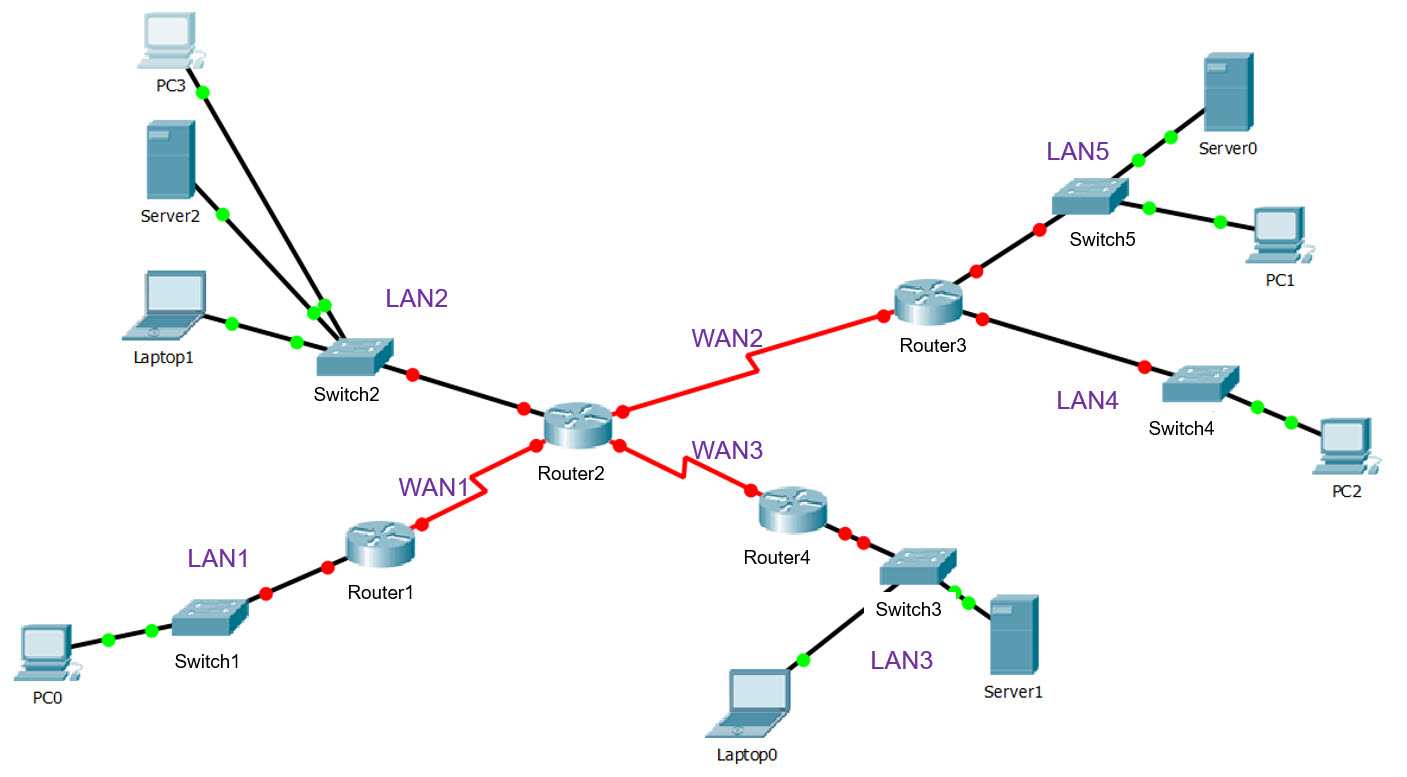
\includegraphics[width=0.95\textwidth]{images/topologie-VLSM.jpg}    
    \caption{Topologie - auto-évaluation (vlsm)}
    \label{}
\end{figure}





\item Sous-réseaux:
\begin{figure}[H]
    \centering
    \begin{tabular}{|c|c|c|c|c|c|} \hline
        &      ip      & bits    & netmask             & réseau              & broadcast           \\ \hline
        LAN2 & 47      & 6       & 255.255.255.1100 0000 & 172.16.54.0000 0000 & 172.16.54.0011 1111 \\
        LAN5 & 26      & 5       & 255.255.255.1110 0000 & 172.16.54.0100 0000 & 172.16.54.0101 1111 \\
        LAN4 & 17      & 5       & 255.255.255.1110 0000 & 172.16.54.0110 0000 & 172.16.54.0111 1111 \\
        LAN1 & 10      & 4       & 255.255.255.1111 0000 & 172.16.54.1000 0000 & 172.16.54.1000 1111 \\
        LAN3 &  8      & 3       & 255.255.255.1111 1000 & 172.16.54.1001 0000 & 172.16.54.1001 0111 \\
        WAN1 &  4      & 2       & 255.255.255.1111 1100 & 172.16.54.1001 1000 & 172.16.54.1001 1011 \\
        WAN2 &  4      & 2       & 255.255.255.1111 1100 & 172.16.54.1001 1100 & 172.16.54.1001 1111 \\
        WAN3 &  4      & 2       & 255.255.255.1111 1100 & 172.16.54.1010 0000 & 172.16.54.1010 0011 \\ \hline
    \end{tabular}
    \caption{Tableau des réseaux (1) - auto-évaluation (vlsm)}
    \label{}
\end{figure}
\textbf{Remarque:} l'adresse réseau et le broadcast sont comprises dans \textit{ip} (= nombre d'ip pour le sous-réseau). \\
\textcolor{red}{\textbf{Attention !}} Le LAN5 a plus d'adresses ip à distribuer mais il a le même netmask que le LAN4, donc le LAN4 aura l'adresse réseau \textit{avant} LAN5 (voir consignes). Les adresses sont donc incorrectes pour les LAN4 et LAN5.
\begin{figure}[H]
    \centering
    \begin{tabular}{|c|c|c|c|} \hline
        &      netmask         & réseau        & broadcast     \\ \hline
        LAN2 & 255.255.255.192 & 172.16.54.0   & 172.16.54.63  \\
        LAN5 & 255.255.255.224 & 172.16.54.64  & 172.16.54.95  \\
        LAN4 & 255.255.255.224 & 172.16.54.96  & 172.16.54.127 \\
        LAN1 & 255.255.255.240 & 172.16.54.128 & 172.16.54.143 \\
        LAN3 & 255.255.255.248 & 172.16.54.144 & 172.16.54.151 \\
        WAN1 & 255.255.255.252 & 172.16.54.152 & 172.16.54.155 \\
        WAN2 & 255.255.255.252 & 172.16.54.156 & 172.16.54.159 \\
        WAN3 & 255.255.255.252 & 172.16.54.160 & 172.16.54.163 \\ \hline
    \end{tabular}
    \caption{Tableau des réseaux (2) - auto-évaluation (vlsm)}
    \label{}
\end{figure}





\item Adresses des interfaces:
\begin{figure}[H]
    \centering
    \begin{tabular}{|c|c| c |c|c|} \hline
        & & netmask & ip & gateway \\ \hline

        \multirow{3}{*}{LAN1}
        & R1  & 255.255.255.240 & 172.16.54.129 & / \\
        & S1  & 255.255.255.240 & 172.16.54.130 & 172.16.54.129 \\
        & PC0 & 255.255.255.240 & 172.16.54.132 & 172.16.54.129 \\ \hline

        \multirow{5}{*}{LAN2}
        & R2  & 255.255.255.192 & 172.16.54.1 & / \\
        & S2  & 255.255.255.192 & 172.16.54.2 & 172.16.54.1 \\
        & L1  & 255.255.255.192 & 172.16.54.3 & 172.16.54.1 \\
        & PC3 & 255.255.255.192 & 172.16.54.4 & 172.16.54.1 \\
        & SV2 & 255.255.255.192 & 172.16.54.62 & 172.16.54.1 \\ \hline

        \multirow{4}{*}{LAN3}
        & R4  & 255.255.255.248 & 172.16.54.145 & / \\
        & S3  & 255.255.255.248 & 172.16.54.146 & 172.16.54.145 \\
        & L0  & 255.255.255.248 & 172.16.54.147 & 172.16.54.145 \\
        & SV3 & 255.255.255.248 & 172.16.54.150 & 172.16.54.145 \\ \hline

        \multirow{3}{*}{LAN4}
        & R3  & 255.255.255.224 & 172.16.54.97 & / \\
        & S4  & 255.255.255.224 & 172.16.54.98 & 172.16.54.97 \\
        & PC2 & 255.255.255.224 & 172.16.54.100 & 172.16.54.97 \\ \hline

        \multirow{4}{*}{LAN5}
        & R3  & 255.255.255.224 & 172.16.54.65 & / \\
        & S5  & 255.255.255.224 & 172.16.54.66 & 172.16.54.65 \\
        & PC1 & 255.255.255.224 & 172.16.54.68 & 172.16.54.65 \\
        & SV0 & 255.255.255.224 & 172.16.54.94 & 172.16.54.65 \\ \hline

        \multirow{2}{*}{WAN1}
        & R1 & 255.255.255.252 & 172.16.54.153 & / \\
        & R2 & 255.255.255.252 & 172.16.54.154 & / \\ \hline

        \multirow{2}{*}{WAN2}
        & R2 & 255.255.255.252 & 172.16.54.157 & / \\
        & R3 & 255.255.255.252 & 172.16.54.158 & / \\ \hline

        \multirow{2}{*}{WAN3}
        & R2 & 255.255.255.252 & 172.16.54.161 & / \\
        & R4 & 255.255.255.252 & 172.16.54.162 & / \\ \hline
    \end{tabular}
    \caption{Tableau des interfaces - auto-évaluation (vlsm)}
    \label{}
\end{figure}





\end{itemize}





Questions:
\begin{itemize}
    \item Quel sera le masque de sous-réseau du réseau LAN1 (sous la forme 32 bits, ex: 255.255.255.0) ?
    \begin{example}
        255.255.255.240
    \end{example}
    \item Quel sera le masque de sous-réseau du réseau LAN2 (sous la forme 32 bits, ex: 255.255.255.0) ?
    \begin{example}
        255.255.255.192
    \end{example}
    \item Quel sera le masque de sous-réseau du réseau LAN3 (sous la forme 32 bits, ex: 255.255.255.0) ?
    \begin{example}
        255.255.255.248
    \end{example}
    \item Quel sera le masque de sous-réseau du réseau LAN4 (sous la forme 32 bits, ex: 255.255.255.0) ?
    \begin{example}
        255.255.255.224
    \end{example}
    \item Quel sera le masque de sous-réseau du réseau LAN5 (sous la forme 32 bits, ex: 255.255.255.0) ?
    \begin{example}
        255.255.255.224
    \end{example}
    \item Quel sera le masque de sous-réseau des réseaux WAN1 / WAN2 / WAN3  (sous la forme 32 bits, ex: 255.255.255.0) ?
    \begin{example}
        255.255.255.252
    \end{example}
    \item Quelle sera l'adresse IP du Router1 sur le LAN1?
    \begin{example}
        172.16.54.129
    \end{example}
    \item Quelle sera l'adresse IP du Switch1?
    \begin{example}
        172.16.54.130
    \end{example}
    \item Quelle sera l'adresse du default gateway du Switch1?
    \begin{example}
        172.16.54.129
    \end{example}
    \item Quelle sera l'adresse IP du PC0?
    \begin{example}
        172.16.54.132
    \end{example}
    \item Quelle sera l'adresse du default gateway du PC0?
    \begin{example}
        172.16.54.129
    \end{example}
    \item Quelle sera l'adresse IP du Router2 sur le LAN2?
    \begin{example}
        172.16.54.1
    \end{example}
    \item Quelle sera l'adresse IP du Server2?
    \begin{example}
        172.16.54.62
    \end{example}
    \item Quelle sera l'adresse IP du Router4 sur le LAN3?
    \begin{example}
        172.16.54.145
    \end{example}
    \item Quelle sera l'adresse IP du Router3 sur le LAN4?
    \begin{example}
        \textcolor{red}{\textbf{Attention !}} La bonne réponse est: 172.16.54.65.
    \end{example}
    \item Quelle sera l'adresse IP du Router3 sur le LAN5?
    \begin{example}
        \textcolor{red}{\textbf{Attention !}} La bonne réponse est: 172.16.54.97.
    \end{example}
    \item Quelle sera l'adresse IP du Router1 sur le WAN1?
    \begin{example}
        172.16.54.153
    \end{example}
    \item Quelle sera l'adresse IP du Router2 sur le WAN1?
    \begin{example}
        172.16.54.154
    \end{example}
    \item Quelle sera l'adresse IP du Router2 sur le WAN2?
    \begin{example}
        172.16.54.157
    \end{example}
    \item Quelle sera l'adresse IP du Router4 sur le WAN3?
    \begin{example}
        172.16.54.162
    \end{example}
\end{itemize}















\section{Labo 8 --- Configurer RIPv2}





Topologie:
\begin{center}
    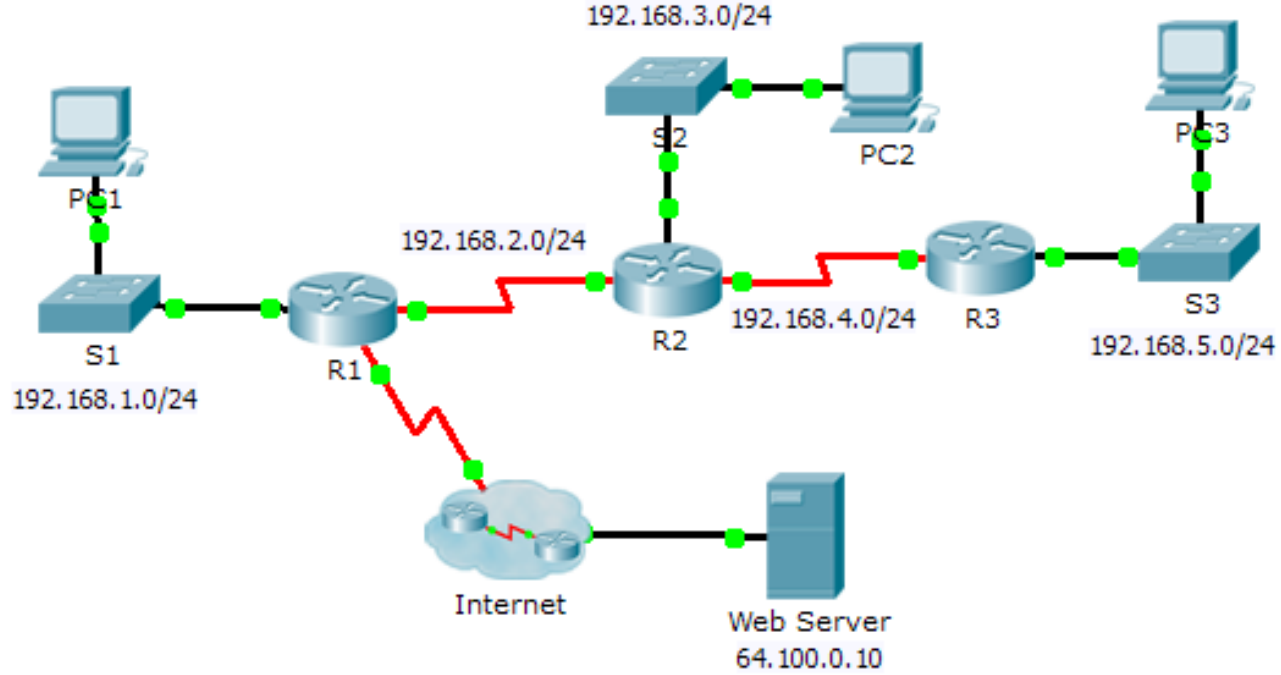
\includegraphics[width=0.85\textwidth]{images/topologie-labo8.PNG}
\end{center}










\subsection{Manipulation}





\begin{itemize}





\item Étape 1: configurer RIPv2 sur R1.
\begin{enumerate}
    \item Utiliser la commande appropriée pour créer une route par défaut sur R1 pour que tout le trafic Internet quitte le réseau via S0/0/1.
    \begin{example}
        \begin{itemize}
            \item \texttt{enable}
            \item \texttt{configure terminal}
            \item \texttt{ip route 0.0.0.0 0.0.0.0 s0/0/1}
        \end{itemize}
    \end{example}
    \item Entrer en mode de configuration du protocole RIP.
    \begin{example}
        \begin{itemize}
            \item \texttt{router rip}
        \end{itemize}
    \end{example}
    \item Utiliser la version 2 du protocole RIP et désactiver la synthèse des réseaux.
    \begin{example}
        \begin{itemize}
            \item \texttt{version 2}
            \item \texttt{no auto-summary}
        \end{itemize}
    \end{example}
    \item Configurer RIP pour les réseaux qui se connectent à R1.
    \begin{example}
        \begin{itemize}
            \item \texttt{network 192.168.1.0}
            \item \texttt{network 192.168.2.0}
        \end{itemize}
    \end{example}
    \item Configurer le port LAN (qui ne contient aucun routeur) afin qu'il n'envoie aucune information de routage.
    \begin{example}
        \begin{itemize}
            \item \texttt{passive-interface g0/0}
        \end{itemize}
    \end{example}
    \item Publier/propager la route par défaut configurée à l'étape 1 avec d'autres routeurs RIP.
    \begin{example}
        \begin{itemize}
            \item \texttt{default-information originate}
        \end{itemize}
    \end{example}
    \item Enregistrer la configuration.
    \begin{example}
        \begin{itemize}
            \item \texttt{end}
            \item \texttt{copy running-config startup-config}
        \end{itemize}
    \end{example}
\end{enumerate}





\item Étape 2: configurer RIPv2 sur R2.
\begin{enumerate}
    \item Entrer en mode de configuration du protocole RIP.
    \begin{example}
        \begin{itemize}
            \item \texttt{enable}
            \item \texttt{configure terminal}
            \item \texttt{router rip}
        \end{itemize}
    \end{example}
    \item Utiliser la version 2 du protocole RIP et désactiver la synthèse des réseaux.
    \begin{example}
        \begin{itemize}
            \item \texttt{version 2}
            \item \texttt{no auto-summary}
        \end{itemize}
    \end{example}
    \item Configurer RIP pour les réseaux directement connectés à R2.
    \begin{example}
        \begin{itemize}
            \item \texttt{network 192.168.2.0}
            \item \texttt{network 192.168.3.0}
            \item \texttt{network 192.168.4.0}
        \end{itemize}
    \end{example}
    \item Configurer l'interface qui ne contient aucun routeur pour qu'elle n'envoie pas d'informations de routage.
    \begin{example}
        \begin{itemize}
            \item trouver l'interface: \texttt{show running-config}, fonctionne après la commande \texttt{enable}
            \item \texttt{passive-interface g0/0}
        \end{itemize}
    \end{example}
    \item Enregistrer la configuration.
    \begin{example}
        \begin{itemize}
            \item \texttt{end}
            \item \texttt{copy running-config startup-config}
        \end{itemize}
    \end{example}
\end{enumerate}





\item Étape 3: configurer RIPv2 sur R3 (répéter l'étape 2 sur R3).
\begin{example}
    \begin{itemize}
        \item \texttt{enable}
        \item \texttt{configure terminal}
        \item \texttt{router rip}

        \item \texttt{version 2}
        \item \texttt{no auto-summary}

        \item \texttt{network 192.168.4.0}
        \item \texttt{network 192.168.5.0}

        \item (\texttt{show running-config})
        \item \texttt{passive-interface g0/0}

        \item \texttt{end}
        \item \texttt{copy running-config startup-config}
    \end{itemize}
\end{example}





\item Clicker sur \textit{Check Results} de la fenêtre \textit{PT Activity} pour voir si tout est complété correctement.
\begin{center}
    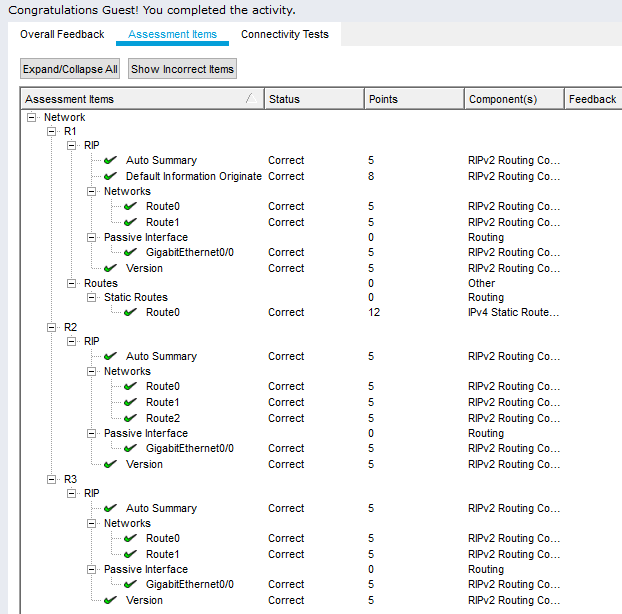
\includegraphics[width=0.65\textwidth]{images/activity-completed1-labo8.PNG}
\end{center}





\end{itemize}










\subsection{Vérification}





\begin{itemize}
    \item Étape 1: Afficher les tables de routage de R1, R2 et R3.
    \begin{example}
        Afficher les tables:
        \begin{itemize}
            \item \texttt{show ip route}
            \item \texttt{show ip route rip}
        \end{itemize}
        Afficher le protocole de routage:
        \begin{itemize}
            \item \texttt{show ip protocols}
        \end{itemize}
        Afficher de la base de donnée du protocole RIP:
        \begin{itemize}
            \item \texttt{show ip rip database}
        \end{itemize}
        \textcolor{red}{\textbf{Attention !}} pour vider la table de routage: \texttt{clear ip route *}.
    \end{example}
    \item Étape 2: Vérifier la connectivité complète vers toutes les destinations.
    \begin{example}
        Command Prompt du PC1:
        \begin{itemize}
            \item PC1-R1: \texttt{ping 192.168.1.1}
            \item PC1-WebServer: \texttt{ping 64.100.0.10}
            \item PC1-PC2: \texttt{ping 192.168.3.10}
            \item PC1-PC3: \texttt{ping 192.168.5.10}
        \end{itemize}
        Command Prompt du PC2:
        \begin{itemize}
            \item PC2-WebServer: \texttt{ping 64.100.0.10}
            \item PC2-PC3: \texttt{ping 192.168.5.10}
        \end{itemize}
        Command Prompt du PC3:
        \begin{itemize}
            \item PC3-WebServer: \texttt{ping 64.100.0.10}
        \end{itemize}
        \textbf{Remarque:} alternatives à la commande \texttt{ping}:
        \begin{itemize}
            \item sur pc: \texttt{tracert}
            \item sur routeur: \texttt{traceroute}
        \end{itemize}
    \end{example}
\end{itemize}
















\section{Labo 9 --- Configurer RIPv2}










\subsection{Préparation}





\begin{itemize}



\item Topologie:
\begin{center}
    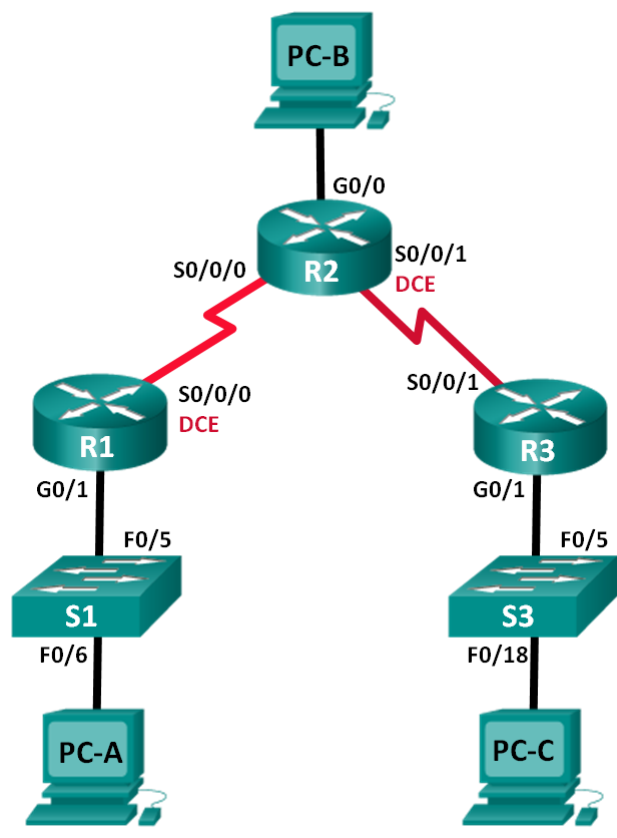
\includegraphics[width=0.5\textwidth]{images/topologie-labo9.PNG}
\end{center}



\item Table d'adressage:
\begin{center}
    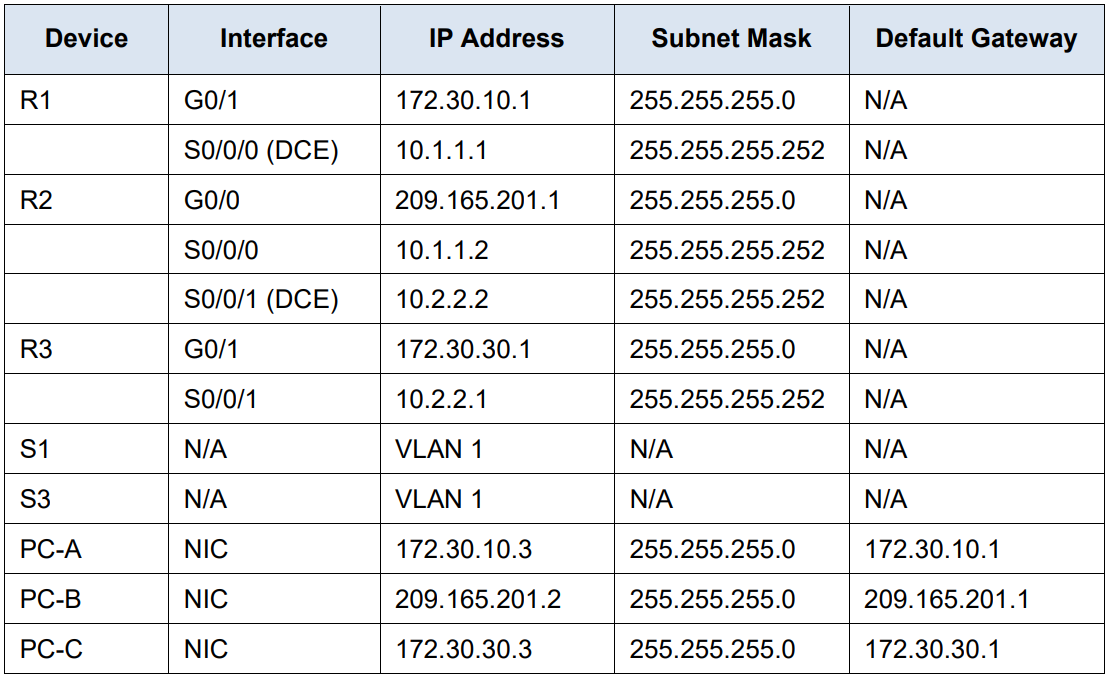
\includegraphics[width=0.85\textwidth]{images/table-adressage-labo9.PNG}
\end{center}



\item Appareils:
\begin{itemize}
    \item routeur: cisco 1941
    \item switch: cisco 2960
    \item pc windows
\end{itemize}



\end{itemize}










\subsection{Manipulation --- Partie 1: construire le réseau et paramètres de base}





\begin{itemize}





\item Étape 1: câbler le réseau comme indiqué dans la topologie.
\begin{center}
    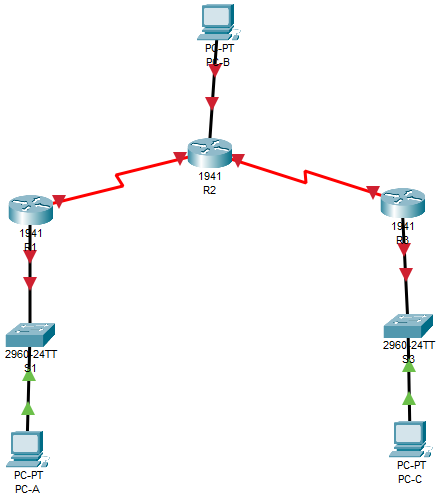
\includegraphics[width=0.5\textwidth]{images/cablage-labo9.PNG}
\end{center}





\item Étape 2: initialiser et recharger les routeurs et les switchs.
\begin{enumerate}
    \item Routeurs:
    \begin{example}
        \begin{itemize}
            \item \texttt{enable}
            \item \texttt{erase startup-config}
            \item \texttt{reload}
        \end{itemize}
    \end{example}
    \item Switchs:
    \begin{example}
        \begin{itemize}
            \item \texttt{enable}
            \item \texttt{delete vlan.dat}
            \item \texttt{erase startup-config}
            \item \texttt{reload}
        \end{itemize}
    \end{example}
\end{enumerate}





\item Étape 3: configurer les paramètres de base pour chaque routeur et switch.
\begin{enumerate}
    \item Désactiver la recherche DNS:
    \begin{example}
        \begin{itemize}
            \item \texttt{enable}
            \item \texttt{configure terminal}
            \item \texttt{no ip domain-lookup}
        \end{itemize}
    \end{example}
    \item Configurer les noms de périphériques comme indiqué dans la topologie:
    \begin{example}
        \begin{itemize}
            \item \texttt{hostname <nom>}
        \end{itemize}
    \end{example}
    \item Configurer le cryptage des mots de passe:
    \begin{example}
        \begin{itemize}
            \item \texttt{service password-encryption}
        \end{itemize}
    \end{example}
    \item Attribuer \textit{class} comme mot de passe EXEC privilégié
    \begin{example}
        \begin{itemize}
            \item \texttt{enable secret class}
        \end{itemize}
    \end{example}
    \item Attribuer \textit{class} comme mot de passe console et vty:
    \begin{example}
        \begin{itemize}
            \item \texttt{line console 0}
            \item \texttt{password cisco}
            \item \texttt{login}
            \item \texttt{line vty 0 4} \qquad (\texttt{line vty 0 15}, pour les switchs)
            \item \texttt{password cisco}
            \item \texttt{login}
            \item \texttt{exit}
        \end{itemize}
    \end{example}
    \item Configurer une bannière MOTD pour avertir les utilisateurs qu'un accès non autorisé est interdit:
    \begin{example}
        \begin{itemize}
            \item \texttt{banner motd \%Authorized access only!\%}
        \end{itemize}
    \end{example}
    \item Configurer la journalisation synchrone (= logging synchronous) pour la ligne de console:
    \begin{example}
        \begin{itemize}
            \item \texttt{line console 0}
            \item \texttt{logging synchronous}
            \item \texttt{exit}
        \end{itemize}
    \end{example}
    \item Configurer les adresses IP répertoriées dans le tableau d'adressage pour toutes les interfaces:
    \begin{example}
        \begin{itemize}
            \item \texttt{interface <interface>}
            \item \texttt{ip address <ip> <netmask>}
            \item \texttt{no shutdown}
        \end{itemize}
    \end{example}
    \item Configurer une description pour chaque interface avec une adresse IP:
    \begin{example}
        \begin{itemize}
            \item \texttt{description <description>}
        \end{itemize}
    \end{example}
    \item Configurer la fréquence d'horloge, le cas échéant, sur l'interface série DCE:
    \begin{example}
        \begin{itemize}
            \item \texttt{clock rate <fréquence\_horloge>}
        \end{itemize}
    \end{example}
    \item Copier la configuration en cours d'exécution dans la configuration de démarrage:
    \begin{example}
        \begin{itemize}
            \item \texttt{end}
            \item \texttt{copy running-config startup-config}
        \end{itemize}
    \end{example}
\end{enumerate}





\item Étape 4: configurer l'adressage IP des PC.





\item Étape 5: tester la connectivité.
\begin{example}
    Command prompt du PC-A (uniquement des réponses du routeur):
    \begin{itemize}
        \item \texttt{ping 209.165.201.2}, ou: \texttt{tracert 209.165.201.2}
        \item \texttt{ping 172.30.30.3}, ou: \texttt{tracert 172.30.30.3}
    \end{itemize}
    Command prompt du PC-B (uniquement des réponses du routeur):
    \begin{itemize}
        \item \texttt{ping 172.30.30.3}, ou: \texttt{tracert 172.30.30.3}
    \end{itemize}
\end{example}





\end{itemize}










\subsection{Manipulation --- Partie 2: configurer et vérifier le routage RIPv2}





\begin{itemize}





\item Étape 1: configurer le routage RIPv2.
\begin{example}
    \begin{itemize}
        \item \texttt{enable}
        \item \texttt{configure terminal}
        \item \texttt{router rip}
        \item \texttt{version 2}
        \item \texttt{network <réseau\_connecté\_au\_routeur>} \qquad (pour chaque réseau)
        \item \texttt{passive-interface <réseau\_connecté\_au\_pc>}
        \item \texttt{end}
    \end{itemize}
\end{example}





\item Étape 2: examiner l'état actuel du réseau.
\begin{example}
    \begin{itemize}
            \item \texttt{show ip interface brief}
            \item \texttt{debug ip rip}
            \item \texttt{undebug all}
            \item \texttt{show ip protocols}
            \item \texttt{show run}
            \item \texttt{show ip route}
        \end{itemize}
\end{example}





\item Étape 3: désactiver le résumé automatique.
\begin{example}
    \begin{itemize}
        \item \texttt{router rip}
        \item \texttt{no auto-summary}
    \end{itemize}
\end{example}





\item Étape 4: configurer et redistribuer un itinéraire par défaut pour l'accès à Internet.
\begin{example}
    Sur \textcolor{red}{\textbf{un seul}} des routeurs:
    \begin{itemize}
        \item \texttt{ip route 0.0.0.0 0.0.0.0 <>} \qquad (ex: sur R2, \texttt{ip route 0.0.0.0 0.0.0.0 209.165.201.2})
        \item \texttt{router rip}
        \item \texttt{default-information originate}
    \end{itemize}
\end{example}





\item Étape 5: vérifiez la configuration du routage.
\begin{example}
    \begin{itemize}
        \item \texttt{show ip route}
    \end{itemize}
\end{example}





\item Étape 6: vérifier la connectivité.
\begin{example}
    \begin{itemize}
        \item Ping entre les PC.
        \item Ping vers internet.
    \end{itemize}
\end{example}





\end{itemize}










\subsection{Questions}





\begin{enumerate}

\item Est-ce que ça change quelque chose si on configure via le terminal en cliquant sur le routeur/switch ou en connectant le PC au port console et en configurant àpd terminal du PC ?

\end{enumerate}





\textbf{Remarques:}
\begin{itemize}
    \item La commande: \texttt{write}, est équivalente à la commande: \texttt{copy running-config startup-config}.
\end{itemize}






























\appendix

























\newpage \section{}





\begin{itemize}





\item Modes:
\begin{center}
    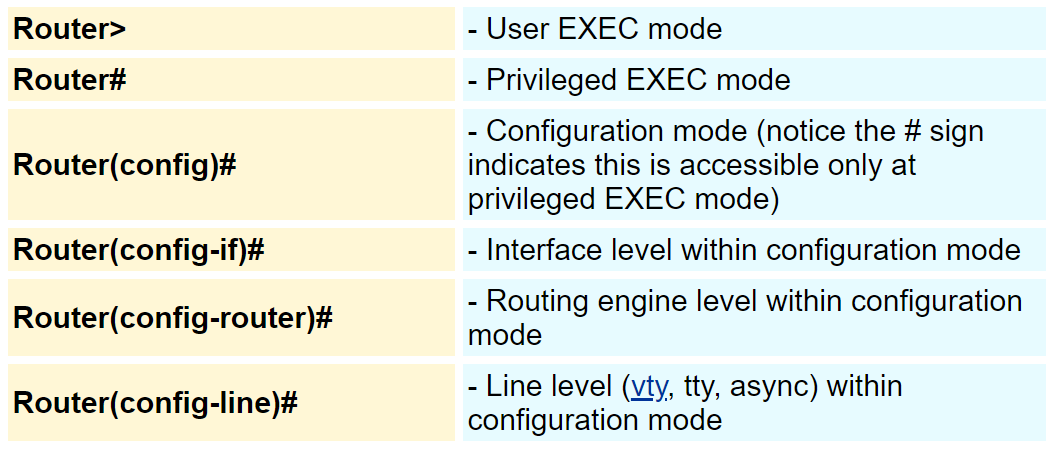
\includegraphics[width=0.65\textwidth]{images/modes01.PNG}
\end{center}





\item Commandes de base:
\begin{itemize}
    \item \texttt{hostname <>}
    \item \texttt{copy running-config startup-config}
    \item \texttt{enable secret <>}
    \item \texttt{service password-encryption}
    \item \texttt{security passwords min-length <>}
    \item \texttt{ip domain-name <>}
    \item \texttt{crypto key generate rsa <>}
    \item \texttt{ip default-gateway <>}
\end{itemize}





\item ...
\begin{itemize}

\item %
\begin{verbatim}
line con 0
password <>
login
exit
\end{verbatim}

\item %
\begin{verbatim}
line vty 0 4
password <>
login
exit
\end{verbatim}

\item %
\begin{verbatim}
line vty 0 4
transport input ssh
login local
\end{verbatim}

\item %
\begin{verbatim}
interface <>
ip address <> <>
no shutdown
exit
\end{verbatim}

\item %
\begin{verbatim}
interface <>
ipv6 address <ip>/<netmask>
ipv6 address <> link-local
no shutdown
exit
\end{verbatim}

\end{itemize}




\end{itemize}










\subsection{}





\textbf{Attention !} Quand on donne une default gateway au switch, c'est pour tout le switch et pas seulement pour une interface.




















\end{document}
